\documentclass[journal]{IEEEtran}
\IEEEoverridecommandlockouts
\usepackage{cite}
\usepackage{amsmath,amssymb,amsfonts}
\usepackage{graphicx}
\usepackage{booktabs}
\usepackage{multirow}
\usepackage{array}
\usepackage{xcolor}
\usepackage{algorithm}
\usepackage{algpseudocode}
\usepackage{tikz}
\usetikzlibrary{positioning,arrows.meta,shapes.geometric,fit,calc}
\usepackage[hidelinks]{hyperref}
\renewcommand{\algorithmicrequire}{\textbf{Input:}}
\renewcommand{\algorithmicensure}{\textbf{Output:}}

\setcounter{topnumber}{4}\setcounter{dbltopnumber}{3}\setcounter{totalnumber}{6}
\renewcommand{\topfraction}{0.92}\renewcommand{\dbltopfraction}{0.92}\renewcommand{\textfraction}{0.06}
\renewcommand{\floatpagefraction}{0.75}\renewcommand{\dblfloatpagefraction}{0.75}

\begin{document}

\title{RL-DOHO: A Dandelion--Hippopotamus Hybrid with Stagnation-Triggered Interventions for Wrapper Feature Selection}

\author{Preetha~Evangeline~D, Prasenjit~Choudhury, Shreyansh~Dabgar, and Aditya~Jha%
\thanks{The authors are with the School of Computer Science and Engineering, Vellore Institute of Technology, Chennai, India. % TODO: add e-mail addresses
Code, notebooks and per-run results: \url{https://github.com/adj-04/rl-doho}.}}

\markboth{Preprint}{Evangeline D \MakeLowercase{\textit{et al.}}: RL-DOHO: Stagnation-Triggered Interventions for Feature Selection}

\maketitle

\begin{abstract}
Population-based wrapper feature selection often stops improving once the population has settled on one subset. We propose RL-DOHO, a hybrid of the Dandelion Optimizer (DO) and Hippopotamus Optimization (HO). It runs DO iterations while the best subset keeps improving. After two iterations without improvement, a UCB1 bandit, rewarded by fitness gain per evaluation, chooses one of four interventions: a tabu-guarded bit-flip search around the best subset, a tabu-guarded restart of the worse half of the population, a DO iteration or an HO iteration. We compared RL-DOHO with the published DO and HO, a fixed DO-then-HO hybrid, a genetic algorithm (GA), binary particle swarm and grey wolf optimizers, LASSO, mRMR, ReliefF and the full feature set, at equal fitness-evaluation budgets and ten seeds, on eleven datasets: a 12,085-patient rheumatic and autoimmune disease dataset, five gene-expression datasets and five medical tabular datasets. Nine hypotheses were fixed before the runs that test them. Over the 110 paired runs, RL-DOHO reached lower fitness than DO in 103 and higher in 4, and was ahead of the fixed hybrid, binary PSO and mRMR significantly more often than behind them. It was level with HO (58 against 49) and had a slightly better average rank within the DO--HO family over all runs, although HO ranked better on repeated train/test splits of the clinical data; the GA reached lower fitness in 85 runs against 22. No test-accuracy difference was significant after correction. The same intervention layer added to HO improved it in 71 runs against 29 ($p<0.001$), but did not change the GA (45 against 49). How the intervention was chosen did not matter: UCB1, tabular Q-learning and random selection were level at the standard budget and at three times the budget. Triggering early did matter, with $\kappa\le2$ better than 3 or 4. On the tabular datasets the bit-flip search alone reached lower fitness than the full set of interventions (39 against 8 runs), but not on gene data (19 against 30, not significant). Repeating the tabular benchmark with a support vector machine instead of 5-NN barely changed the ranking of the methods (Spearman 0.99) and reproduced the comparisons with DO, HO and the GA, the effect of the intervention layer on HO and the GA, and the advantage of the bit-flip search alone. Repeated over three train/test splits of the clinical data, RL-DOHO differed significantly only from DO and the full feature set. On the clinical and tabular data RL-DOHO evaluated 35--40\% fewer distinct subsets than HO or the GA, which makes it cheaper when fitness evaluations dominate the cost.
\end{abstract}

\begin{IEEEkeywords}
feature selection, metaheuristics, dandelion optimizer, hippopotamus optimization, stagnation, multi-armed bandit, Q-learning, rheumatic disease, gene expression
\end{IEEEkeywords}

%% ======================================================================
\section{Introduction}

Feature selection asks which subset of the measured variables a classifier should use. Smaller subsets are cheaper to collect, easier to interpret and, when irrelevant variables are removed, often more accurate. Wrapper methods score each candidate subset by training a classifier on it. This ties the selection to the model that will be used, but turns the problem into a search over $2^D-1$ subsets for $D$ features~\cite{kohavi1997,xue2016}. Population-based metaheuristics are a common choice for this search because they need only fitness values.

Two recent algorithms motivated this work. The Dandelion Optimizer (DO)~\cite{zhao2022do} moves its population through rising, descending and landing stages. Hippopotamus Optimization (HO)~\cite{amiri2024ho} combines moves towards the dominant solution, random defensive jumps and a local escape step, with greedy acceptance. Both were designed for continuous problems. When their positions are mapped to feature subsets, the population can stop producing new subsets long before the evaluation budget runs out. This suggests a hybrid that keeps one algorithm's moves while they work and intervenes when progress stops. Because the right intervention is not known in advance, we let a UCB1 multi-armed bandit~\cite{auer2002} choose it. A bandit is the stateless case of reinforcement learning~\cite{sutton2018}, which is where the method's name, RL-DOHO, comes from.

The method was developed for a recently released dataset of 12,085 patients with six autoimmune rheumatic diseases or no disease, described by 14 routine clinical and laboratory variables~\cite{mahdi2025data}. Because a 14-feature problem is small, we also evaluated it on five gene-expression datasets with 2,000--7,129 candidate features and on five medical tabular datasets with 19--44 features.

This paper makes five contributions:
\begin{itemize}
\item We describe RL-DOHO. It combines the published DO and HO update rules with stagnation-triggered interventions (bit-flip search and restarts, both with tabu memory), a UCB1 operator selector rewarded by fitness gain per evaluation, and a sparse initial population for high-dimensional data.
\item We compare it with ten alternatives on eleven datasets of three kinds under equal fitness-evaluation budgets: its parent algorithms, a fixed-switch hybrid, three established wrapper metaheuristics, three filter or embedded methods and the full feature set. On the clinical data we repeat the comparison on further train/test splits.
\item We fixed eight hypotheses and their tests before running the experiments that test them, and we report all eight outcomes.
\item We separate the parts of the method. Ablations compare three controllers (UCB1, tabular Q-learning and random selection) at the standard and at three times the budget, vary the stagnation trigger, and attach the same intervention layer to HO and to the GA. We repeat the tabular benchmark with a second classifier (SVM), and report what each method costs in distinct fitness evaluations and in algorithm overhead.
\item We report a sensitivity analysis against an earlier version of this study, which used simplified DO and HO update rules and a dense initial population.
\end{itemize}

In short, RL-DOHO improves clearly on DO and on a fixed DO-then-HO hybrid. It is level with HO and was almost never the worst of the DO--HO family, but a GA reached lower fitness more often. The improvement comes from intervening when the search stalls, not from how the intervention is chosen: the intervention layer also improves HO, and a random choice of intervention works as well as a learned one. On the tabular datasets, with 19--44 features, a simple bit-flip search around the best subset does better on its own than the full set of interventions, under both classifiers we tested; on gene data, with thousands of features, it is not (the full set was ahead, though not significantly). Section~\ref{sec:related} reviews related work, Section~\ref{sec:method} describes the method, Section~\ref{sec:setup} the protocol and Section~\ref{sec:results} the results. Section~\ref{sec:discussion} discusses them and the limitations of the study.

%% ======================================================================
\section{Related Work}\label{sec:related}

\subsection{Wrapper feature selection with metaheuristics}
Surveys of evolutionary feature selection~\cite{xue2016} show that genetic algorithms, particle swarm optimization (PSO) and grey wolf optimization (GWO) are among the most used wrapper searches. Binary versions of PSO~\cite{kennedy1997} and GWO~\cite{mirjalili2014gwo,emary2016bgwo} map continuous positions to bits through transfer functions. Hybrids that add local search to a population method are also common; for example, the whale optimization algorithm has been combined with simulated annealing~\cite{mafarja2017}. The no-free-lunch theorems~\cite{wolpert1997} imply that no search method will win on every problem. This is one argument for adaptive hybrids, and also a reason to test them against simple baselines. Reviews of feature selection for cancer classification find that evolutionary and swarm methods remain the dominant wrapper choices on gene-expression data~\cite{ramadhani2025}.

\subsection{The Dandelion and Hippopotamus optimizers}
DO was introduced for continuous engineering problems~\cite{zhao2022do}, and a recent review catalogues its variants and applications~\cite{zhao2026review}. Tang et al. hybridized DO with PSO for engineering design~\cite{tang2024psodo}. In medical applications, DO has been used to select fused deep features for gastrointestinal disease diagnosis~\cite{kiziloluk2024} and to tune the hyperparameters of a network for laryngeal cancer images~\cite{alzakari2024}. HO~\cite{amiri2024ho} has been extended with chaotic initialization and diversity strategies~\cite{pei2025}. Binary variants have been used for feature selection with a random-forest evaluator~\cite{ardiyansa2025} and with multiple perturbation and screening strategies~\cite{yuan2025msho}. The closest work to ours is Q2HO-MFTV~\cite{hashjin2025q2ho}, in which Q-learning selects search strategies inside a binary HO for feature selection. To our knowledge, DO and HO have not previously been combined in a single optimizer.

\subsection{Learning-based operator selection}
Choosing which operator to apply during a run is known as adaptive operator selection, a form of parameter control~\cite{karafotias2015}. Bandit-based selectors, typically UCB variants, are a standard approach~\cite{fialho2010}. Q-learning~\cite{watkins1992} has been used to pick search strategies in a comprehensive-learning GWO for feature selection~\cite{hu2023rlgwo}, in a binary HO~\cite{hashjin2025q2ho}, and to pick perturbation operators in an iterated greedy algorithm for scheduling~\cite{karimi2023}. A practical question for any such controller is whether it beats a random or fixed choice under the budget actually available; we test this directly for a bandit and for a tabular Q-learner.

\subsection{Rheumatic and autoimmune disease data}
The dataset used here was released in 2025 by Mahdi et al.~\cite{mahdi2025data}, who also applied fuzzy evaluation and explainable machine learning to it~\cite{mahdi2025fuzzy}. A clustered binary GWO has been used to select genes linking non-Hodgkin lymphomas with rheumatologic diseases~\cite{karadayi2025}. We are not aware of a published wrapper-metaheuristic feature-selection study on the 2025 rheumatic dataset.

%% ======================================================================
\section{Method}\label{sec:method}

\begin{figure*}[t]
\centering
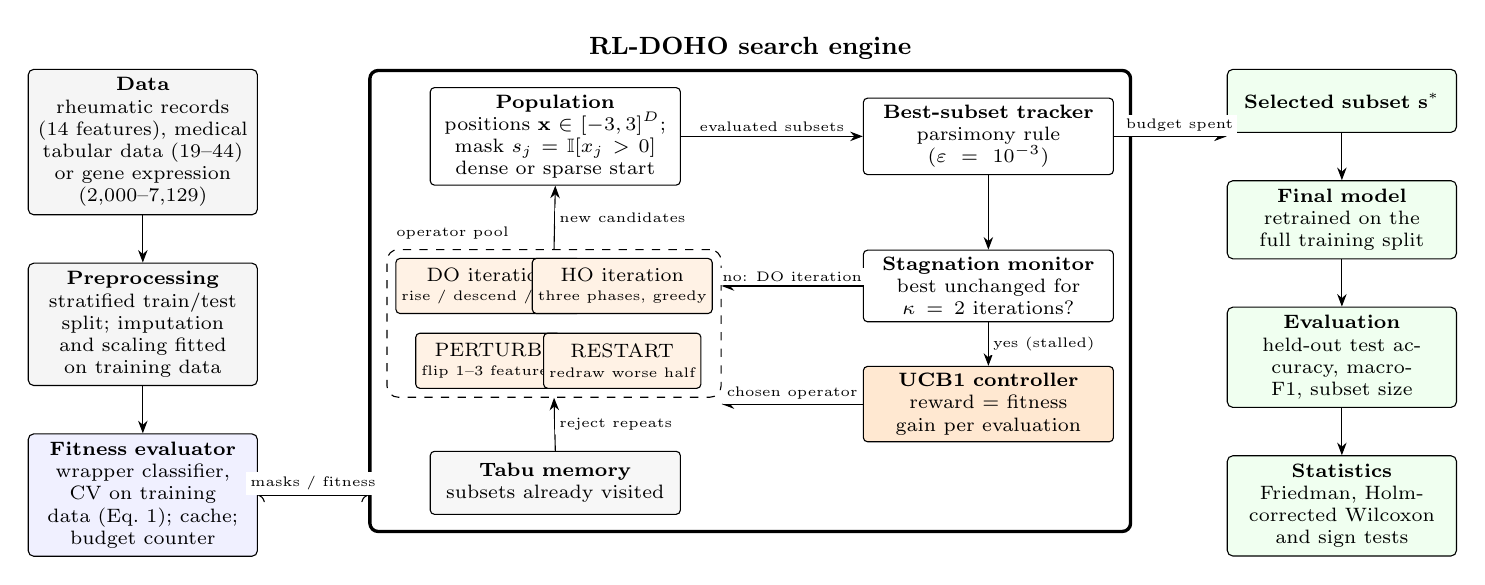
\begin{tikzpicture}[
  font=\scriptsize,
  blk/.style={draw, rounded corners=2pt, align=center, inner sep=3pt, minimum height=8mm, text width=27mm},
  cmp/.style={draw, rounded corners=1.5pt, align=center, inner sep=2.5pt, minimum height=8mm, text width=30mm, fill=white},
  op/.style={draw, rounded corners=1.5pt, align=center, inner sep=2pt, minimum height=7mm, minimum width=15mm, fill=orange!10},
  ar/.style={-{Stealth[length=1.6mm]}, thin},
  lab/.style={font=\tiny, inner sep=1.5pt, fill=white}]
% ---- engine internals (grid: left column x=0, right column x=55mm)
\node[cmp] (pop) at (0,0) {\textbf{Population}\\ positions $\mathbf{x}\in[-3,3]^D$; mask $s_j=\mathbb{I}[x_j>0]$\\ dense or sparse start};
\node[cmp] (track) at (55mm,0) {\textbf{Best-subset tracker}\\ parsimony rule ($\varepsilon=10^{-3}$)};
\node[op] (do) at (-8.5mm,-19mm) {DO iteration\\[-1pt]\tiny rise / descend / land};
\node[op] (ho) at (8.5mm,-19mm) {HO iteration\\[-1pt]\tiny three phases, greedy};
\node[op] (pert) at (-8.5mm,-28.5mm) {PERTURB\\[-1pt]\tiny flip 1--3 features};
\node[op] (rest) at (8.5mm,-28.5mm) {RESTART\\[-1pt]\tiny redraw worse half};
\node[draw, dashed, rounded corners, fit=(do)(ho)(pert)(rest), inner sep=3pt] (pool) {};
\node[font=\tiny, anchor=south west] at (pool.north west) {operator pool};
\node[cmp] (stag) at (55mm,-19mm) {\textbf{Stagnation monitor}\\ best unchanged for $\kappa=2$ iterations?};
\node[cmp, fill=orange!18] (ucb) at (55mm,-34mm) {\textbf{UCB1 controller}\\ reward = fitness gain per evaluation};
\node[cmp, fill=gray!6] (tabu) at (0,-44mm) {\textbf{Tabu memory}\\ subsets already visited};
\node[draw, very thick, rounded corners=3pt, fit=(pop)(track)(pool)(stag)(ucb)(tabu), inner sep=6pt] (engine) {};
\node[font=\small\bfseries, anchor=south] at (engine.north) {RL-DOHO search engine};
% internal arrows
\draw[ar] (pool.north) -- node[lab, right]{new candidates} (pop.south);
\draw[ar] (pop.east) -- node[lab, above]{evaluated subsets} (track.west);
\draw[ar] (track.south) -- (stag.north);
\draw[ar] (stag.south) -- node[lab, right]{yes (stalled)} (ucb.north);
\draw[ar] (stag.west) -- node[lab, above]{no: DO iteration} (pool.east |- stag.west);
\draw[ar] (ucb.west) -- node[lab, above]{chosen operator} (pool.east |- ucb.west);
\draw[ar] (tabu.north) -- node[lab, right]{reject repeats} (pool.south);
% ---- left: data, preprocessing, evaluator
\node[blk, fill=gray!8, anchor=north east] (data) at ([xshift=-14mm]engine.north west) {\textbf{Data}\\ rheumatic records (14 features), medical tabular data (19--44) or gene expression (2,000--7,129)};
\node[blk, fill=gray!8, below=6mm of data] (prep) {\textbf{Preprocessing}\\ stratified train/test split; imputation and scaling fitted on training data};
\node[blk, fill=blue!6, below=6mm of prep] (fit) {\textbf{Fitness evaluator}\\ wrapper classifier, CV on training data (Eq.~1); cache; budget counter};
\draw[ar] (data) -- (prep); \draw[ar] (prep) -- (fit);
\draw[ar, <->] (fit.east) -- node[lab, above]{masks / fitness} (fit.east -| engine.west);
% ---- right: outputs
\node[blk, fill=green!6, anchor=north west] (best) at ([xshift=12mm]engine.north east) {\textbf{Selected subset} $\mathbf{s}^\ast$};
\node[blk, fill=green!6, below=6mm of best] (final) {\textbf{Final model}\\ retrained on the full training split};
\node[blk, fill=green!6, below=6mm of final] (test) {\textbf{Evaluation}\\ held-out test accuracy, macro-F1, subset size};
\node[blk, fill=green!6, below=6mm of test] (stats) {\textbf{Statistics}\\ Friedman, Holm-corrected Wilcoxon and sign tests};
\draw[ar] (best) -- (final); \draw[ar] (final) -- (test); \draw[ar] (test) -- (stats);
\draw[ar] (track.east) -- (track.east -| engine.east) -- node[lab, above]{budget spent} (best.west |- track.east);
\end{tikzpicture}
\caption{Architecture of the feature-selection pipeline. The data are split and preprocessed, and every candidate subset is scored by the wrapper fitness on the training data only, with a cache and a counter that enforces the evaluation budget. Inside the RL-DOHO engine, the population is updated by published DO iterations while the best subset improves. When the stagnation monitor detects $\kappa=2$ stalled iterations, the UCB1 controller chooses one operator from the pool, rewarded by the fitness gain per evaluation, and tabu memory rejects subsets already visited. When the budget is spent, the selected subset is used to retrain the final classifier, which is evaluated on held-out data.}
\label{fig:arch}
\end{figure*}

Fig.~\ref{fig:arch} shows the overall pipeline; the components are described below.

\subsection{Problem formulation and budget}
Let $D$ be the number of candidate features and $\mathbf{s}\in\{0,1\}^D$ a selection mask with $|\mathbf{s}|$ selected features. Every method minimizes
\begin{equation}
f(\mathbf{s}) = \alpha\,\bigl(1-A_{\mathrm{CV}}(\mathbf{s})\bigr) + \beta\,\frac{|\mathbf{s}|}{D}, \qquad \alpha=0.99,\ \beta=0.01,
\label{eq:fitness}
\end{equation}
where $A_{\mathrm{CV}}$ is the cross-validated accuracy (balanced accuracy for GSE93272 and the five medical tabular datasets) of the wrapper classifier on the training data only, and $f=1$ for the empty mask. The fitness is deterministic for a given mask, so repeated masks are served from a cache. Every search method receives the same budget $B$ of fitness evaluations, counted as calls whether or not the mask is cached. We fix the budget in evaluations rather than iterations because HO evaluates about three times as many candidates per iteration as DO.

\subsection{Encoding and initialization}
Each agent holds a position $\mathbf{x}\in[-3,3]^D$, and its mask is $s_j=\mathbb{I}[\sigma(x_j)>0.5]$, where $\sigma$ is the logistic function; equivalently, feature $j$ is selected when $x_j>0$. With the \emph{dense} start, positions are drawn uniformly in $[-1,1]^D$, so each feature starts selected with probability 0.5. For the gene-expression data ($D>100$) all wrapper methods use a \emph{sparse} start instead. Agent $i$ keeps a fraction $p_i$ of the features, drawn log-uniformly between $\min(10/D,0.1)$ and $0.1$, so initial subsets range from about ten features to 10\% of them. Selected coordinates are drawn from $\mathcal{U}(0.1,1)$ and the others from $\mathcal{U}(-1,-0.1)$.

\subsection{Published DO and HO update rules}
\emph{Dandelion Optimizer.} Following~\cite{zhao2022do}, every DO iteration applies three stages to the whole population, with $t$ the iteration, $T$ the number of iterations the budget allows, $\mathbf{x}^\ast$ the elite and $\alpha=r\,(t^2/T^2-2t/T+1)$ with $r\sim\mathcal{U}(0,1)$. In the rising stage, with probability $P(\mathcal{N}(0,1)<1.5)\approx0.93$,
\begin{equation}
\mathbf{x}\leftarrow\mathbf{x}+\alpha\,v_xv_y\,\ln Y\,(\mathbf{x}_s-\mathbf{x}),
\end{equation}
where $\mathbf{x}_s$ is a random point in the search space, $v_x=r_\theta\cos\theta$, $v_y=r_\theta\sin\theta$, $r_\theta=e^{-\theta}$ with $\theta\sim\mathcal{U}(-\pi,\pi)$, and $\ln Y$ is the lognormal density evaluated at $|\mathcal{N}(0,1)|$. Otherwise the position is shrunk, $\mathbf{x}\leftarrow k\,\mathbf{x}$, with the schedule $k$ of~\cite{zhao2022do}. In the descending stage, $\mathbf{x}\leftarrow\mathbf{x}-\alpha\boldsymbol{\beta}\odot(\bar{\mathbf{x}}-\alpha\boldsymbol{\beta}\odot\mathbf{x})$, with $\boldsymbol{\beta}\sim\mathcal{N}(0,1)^D$ and $\bar{\mathbf{x}}$ the population mean. In the landing stage,
\begin{equation}
\mathbf{x}\leftarrow\mathbf{x}^\ast+\mathrm{L\acute{e}vy}\odot\alpha\,(\mathbf{x}^\ast-\delta\,\mathbf{x}),\qquad \delta=2t/T,
\end{equation}
where the Lévy steps use exponent 1.5 and scale 0.01. Each DO iteration costs $N$ evaluations for a population of $N$.

\emph{Hippopotamus Optimization.} Following~\cite{amiri2024ho}, every HO iteration has three phases with greedy acceptance of each candidate. In phase~1 (first half of the population), each agent generates a ``male'' candidate $\mathbf{x}+r(\mathbf{x}^{D}-I_1\mathbf{x})$ towards the dominant agent $\mathbf{x}^{D}$, and a ``female or immature'' candidate. While $e^{-t/T}>0.6$ that candidate moves relative to the mean $\mathbf{m}_G$ of a random group of agents, as $\mathbf{x}+\mathbf{h}_1\odot(\mathbf{x}^{D}-I_2\mathbf{m}_G)$; later it is either $\mathbf{x}+\mathbf{h}_2\odot(\mathbf{m}_G-\mathbf{x}^{D})$ or a random point. Here $I_1,I_2\in\{1,2\}$ and $\mathbf{h}$ is drawn from the five options of~\cite{amiri2024ho}. In phase~2 (second half), a random predator position is evaluated, and the agent jumps relative to it with a Lévy step (scale 0.05) and a distance-dependent term. In phase~3 (all agents), each agent makes a local move inside bounds that shrink as $1/t$. An HO iteration costs about $3N$ evaluations, including the predator evaluations. The original papers leave some details open, such as the size of the random group behind $\mathbf{m}_G$, for which we draw a random size between 1 and $N$; our implementation is in the repository.

\subsection{RL-DOHO}
RL-DOHO (Fig.~\ref{fig:flow}, Algorithm~\ref{alg:rldoho}) applies DO iterations while the best subset keeps improving. A stagnation counter $c$ counts consecutive iterations without an accepted change of the best subset. When $c$ reaches $\kappa=2$, a controller selects one of four arms for the next step:
\begin{itemize}
\item \textbf{PERTURB}: each agent in the worse half is replaced by a copy of the best position with $k\sim\mathcal{U}\{1,2,3\}$ randomly chosen features flipped. Each flipped coordinate is set to the opposite sign, with magnitude from $\mathcal{U}(0.5,2)$. This is a bit-flip local search around the best subset ($N/2$ evaluations).
\item \textbf{RESTART}: each agent in the worse half is redrawn from the initial distribution ($N/2$ evaluations).
\item \textbf{DO}: one DO iteration ($N$ evaluations).
\item \textbf{HO}: one HO iteration (about $3N$ evaluations).
\end{itemize}
PERTURB and RESTART draw candidates through a tabu memory that stores every subset the population has held during the run (HO's predator points are evaluated but not stored). A draw whose mask is already in the memory is redrawn, up to 20 times, after which the last draw is kept. The DO and HO schedules follow the fraction of the budget already spent, so that, for example, DO reaches its landing behaviour at the end of the budget whichever arms were used.

\emph{Controller.} The controller is a UCB1 bandit~\cite{auer2002}. Each arm is pulled once in random order, and afterwards the arm
\begin{equation}
a_t=\arg\max_a\Bigl[\bar{Q}_a + \sqrt{\tfrac{2\ln N_t}{n_a}}\Bigr]
\end{equation}
is chosen, where $\bar{Q}_a$ is the mean reward of arm $a$, $n_a$ its pull count and $N_t=\sum_a n_a$. The reward of a pull is
\begin{equation}
r_t=0.8\,\min\!\Bigl(1,\frac{g_t}{g_{\max}}\Bigr)+0.2\,\frac{1}{|I_t|}\sum_{i\in I_t}\mathbb{I}\bigl[f_i<\tilde f_{t-1}\bigr],
\label{eq:reward}
\end{equation}
where $g_t$ is the decrease in the best fitness divided by the evaluations the step used, $g_{\max}$ is the largest such value observed so far in the run, $I_t$ is the set of agents the arm changed, and $\tilde f_{t-1}$ is the median fitness before the step. A step that only replaces the best subset by one with fewer features, without lowering its fitness, therefore earns no gain term. An earlier reward, 1 for any accepted change and otherwise the median term alone, is kept as an ablation.

\emph{Acceptance.} RL-DOHO keeps the parsimony rule of the earlier version. A candidate replaces the incumbent if its fitness is lower by more than $\varepsilon=10^{-3}$, or if it is within $\varepsilon$ and uses fewer features (or the same number with lower fitness). In the clinical runs, where it was tested, this rule never changed an outcome (Section~\ref{sec:ablation}).

\emph{Q-learning controller (ablation).} To test whether a controller with state does better than the stateless bandit, we also ran RL-DOHO with tabular one-step Q-learning~\cite{watkins1992}. The state combines the budget phase (first, middle or last third of the budget) with whether the previous intervention lowered the best fitness, giving six states. The actions are the four arms and the reward is (\ref{eq:reward}). The learning rate is 0.3, the discount factor 0.5, exploration is $\varepsilon$-greedy with probability 0.2, and the Q-table starts at zero in every run. These settings were fixed before the runs and not tuned.

\begin{figure}[t]
\centering
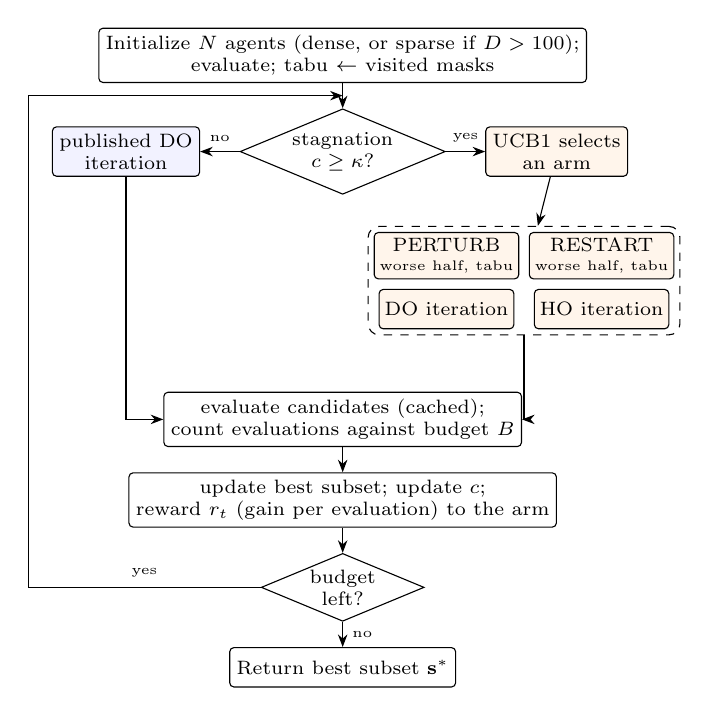
\begin{tikzpicture}[
  node distance=3.2mm and 3mm,
  box/.style={draw, rounded corners=1.5pt, align=center, font=\scriptsize, inner sep=2.5pt, minimum height=5mm},
  dec/.style={draw, diamond, aspect=2.4, align=center, font=\scriptsize, inner sep=0.6pt},
  arm/.style={draw, rounded corners=1.5pt, align=center, font=\scriptsize, inner sep=2pt, fill=orange!8, minimum width=12mm, minimum height=5mm},
  ar/.style={-{Stealth[length=1.6mm]}, thin}]
\node[box] (init) {Initialize $N$ agents (dense, or sparse if $D>100$);\\ evaluate; tabu $\leftarrow$ visited masks};
\node[dec, below=of init] (stag) {stagnation\\ $c\ge\kappa$?};
\node[box, left=5mm of stag, fill=blue!5] (do) {published DO\\ iteration};
\node[box, right=5mm of stag, fill=orange!8] (ucb) {UCB1 selects\\ an arm};
\node[arm, below=7mm of ucb, xshift=-14mm] (pert) {PERTURB\\[-1pt]\tiny worse half, tabu};
\node[arm, right=1.2mm of pert] (rest) {RESTART\\[-1pt]\tiny worse half, tabu};
\node[arm, below=1.2mm of pert] (doa) {DO iteration};
\node[arm, below=1.2mm of rest] (hoa) {HO iteration};
\node[draw, dashed, rounded corners, fit=(pert)(rest)(doa)(hoa), inner sep=2pt] (arms) {};
\node[box, below=25mm of stag] (eval) {evaluate candidates (cached);\\ count evaluations against budget $B$};
\node[box, below=of eval] (acc) {update best subset; update $c$;\\ reward $r_t$ (gain per evaluation) to the arm};
\node[dec, below=of acc] (stop) {budget\\ left?};
\node[box, below=of stop] (out) {Return best subset $\mathbf{s}^\ast$};
\draw[ar] (init) -- (stag);
\draw[ar] (stag) -- node[above, font=\tiny]{no} (do);
\draw[ar] (stag) -- node[above, font=\tiny]{yes} (ucb);
\draw[ar] (ucb) -- (arms);
\draw[ar] (do) |- (eval);
\draw[ar] (arms.south) |- (eval.east);
\draw[ar] (eval) -- (acc);
\draw[ar] (acc) -- (stop);
\draw[ar] (stop) -- node[right, font=\tiny]{no} (out);
\coordinate (mid) at ($(init.south)!0.5!(stag.north)$);
\draw[ar] (stop.west) -- ($(stop.west -| do.west)+(-3mm,0)$) node[pos=0.5, above, font=\tiny]{yes} |- (mid);
\end{tikzpicture}
\caption{Flow of one RL-DOHO run. Published DO iterations are used while the best subset improves; after $\kappa=2$ iterations without an accepted change, the UCB1 controller chooses one of four arms for the next step. The run stops when the evaluation budget is spent.}
\label{fig:flow}
\end{figure}

\begin{algorithm}[t]
\caption{RL-DOHO}\label{alg:rldoho}
\small
\begin{algorithmic}[1]
\Require population $N$, evaluation budget $B$, trigger $\kappa$
\State initialize positions (dense or sparse), evaluate, record best; tabu $\mathcal{T}\leftarrow$ visited masks; $c\leftarrow0$
\While{evaluations used $<B$}
  \If{$c<\kappa$} \State apply one published DO iteration to all agents
  \Else \State $a\leftarrow$ UCB1 choice among \{PERTURB, RESTART, DO, HO\}
    \If{$a\in$ \{PERTURB, RESTART\}} \State redraw the worse half with arm $a$, rejecting masks in $\mathcal{T}$
    \Else \State apply one published DO or HO iteration \EndIf
  \EndIf
  \State evaluate new candidates; add their masks to $\mathcal{T}$; update the best subset
  \State $c\leftarrow0$ if the best subset changed, else $c\leftarrow c+1$
  \If{an arm was pulled} \State give it reward $r_t$ from (\ref{eq:reward}) \EndIf
\EndWhile
\Ensure best mask $\mathbf{s}^\ast$
\end{algorithmic}
\end{algorithm}

\subsection{Fixed-switch hybrid (DOHO)}
To separate the effect of adaptive control from that of simply combining the two algorithms, DOHO runs the published DO for the first half of the evaluation budget and the published HO for the second half. It has no stagnation trigger, local search, tabu memory or bandit.

\subsection{The intervention layer on other optimizers (GA+SI, HO+SI)}
To test whether the interventions help optimizers other than DO, we wrapped the same layer around the GA and around the published HO, which we call GA+SI and HO+SI (SI for stagnation-triggered interventions). The base optimizer runs while the best subset improves. After $\kappa=2$ stalled iterations, UCB1 with the gain reward chooses among PERTURB, RESTART and one iteration of the base optimizer, with the same tabu memory and acceptance rule as RL-DOHO. GA children are stored as positions $\pm1$ so that PERTURB and RESTART can act on them. One HO iteration costs about $3N$ evaluations against $N$ for a GA generation, so HO+SI stalls, and therefore intervenes, less often than GA+SI within the same budget.


%% ======================================================================
\section{Experimental Setup}\label{sec:setup}

\subsection{Datasets}
Table~\ref{tab:data} lists the datasets. The rheumatic dataset~\cite{mahdi2025data} contains 12,085 records collected between 2019 and 2024 from one hospital and three diagnostic laboratories in Iraq. It has seven classes: rheumatoid arthritis (2,848), ankylosing spondylitis (2,127), Sj\"ogren's syndrome (1,852), psoriatic arthritis (1,783), no disease (1,604), systemic lupus erythematosus (1,355) and reactive arthritis (516). Its 14 features are age, gender, ESR, CRP, RF, anti-CCP, C3, C4, HLA-B27, ANA, anti-Ro, anti-La, anti-dsDNA and anti-Sm. Missing values are frequent, from 9\% (ESR) to 43\% (anti-Sm); age and gender are complete (Fig.~\ref{fig:eda}).

The four microarray datasets come from the scikit-feature repository~\cite{li2017fs} and originate from colon tumour~\cite{alon1999}, leukaemia~\cite{golub1999}, lung carcinoma~\cite{bhattacharjee2001} and glioma~\cite{nutt2003} studies. GSE93272 is a whole-blood expression series from patients with rheumatoid arthritis and healthy controls~\cite{tasaki2018}. Several of its 275 samples are repeat samples from the same individual, so we kept the first sample of each individual (101 people: 66 RA, 35 controls).

The five medical tabular datasets were taken from the PMLB collection~\cite{olson2017pmlb}, which provides cleaned copies of UCI datasets. They cover breast tumour diagnosis from cell-nucleus features (WDBC~\cite{street1993}; 357 benign, 212 malignant), hepatitis survival (Hepatitis; 123 and 32 patients), the differential diagnosis of six erythemato-squamous skin diseases (Dermatology~\cite{guvenir1998}; 20--112 patients per class), cardiac SPECT images summarized as region-of-interest features (SPECTF~\cite{kurgan2001}; 254 abnormal, 95 normal) and back-pain outcome (Backache; 155 and 25 patients). We chose them, before running any method on them, as openly available medical classification problems with 19--44 features, a range that lies between the clinical and the gene-expression data. Most of them are imbalanced (minority classes of 14--37\% in the binary ones), so these datasets and GSE93272 use balanced accuracy.

\begin{table}[t]
\centering
\caption{Datasets}
\label{tab:data}
\footnotesize
\setlength{\tabcolsep}{4pt}
\begin{tabular}{@{}lrrrl@{}}
\toprule
Dataset & Samples & Features & Classes & Test set \\
\midrule
Rheumatic~\cite{mahdi2025data} & 12,085 & 14 & 7 & 2,417$^\ddagger$ \\
\midrule
Colon~\cite{alon1999} & 62 & 2,000 & 2 & 19 (per seed) \\
ALL/AML~\cite{golub1999} & 72 & 7,129 & 2 & 22 (per seed) \\
Lung~\cite{bhattacharjee2001} & 203 & 3,312 & 5 & 61 (per seed) \\
Glioma~\cite{nutt2003} & 50 & 4,434 & 4 & 15 (per seed) \\
GSE93272~\cite{tasaki2018} & 101 & 5,000$^\dagger$ & 2 & 31 (per seed) \\
\midrule
WDBC~\cite{street1993} & 569 & 30 & 2 & 171 (per seed) \\
Hepatitis~\cite{olson2017pmlb} & 155 & 19 & 2 & 47 (per seed) \\
Dermatology~\cite{guvenir1998} & 366 & 34 & 6 & 110 (per seed) \\
SPECTF~\cite{kurgan2001} & 349 & 44 & 2 & 105 (per seed) \\
Backache~\cite{olson2017pmlb} & 180 & 32 & 2 & 54 (per seed) \\
\bottomrule
\multicolumn{5}{@{}l@{}}{\scriptsize $^\dagger$Most variable of 54,613 probes, chosen on each training split.}\\
\multicolumn{5}{@{}l@{}}{\scriptsize $^\ddagger$One fixed split for the main runs; two further splits in Section~\ref{sec:splits}.}
\end{tabular}
\end{table}

\begin{figure*}[t]
\centering
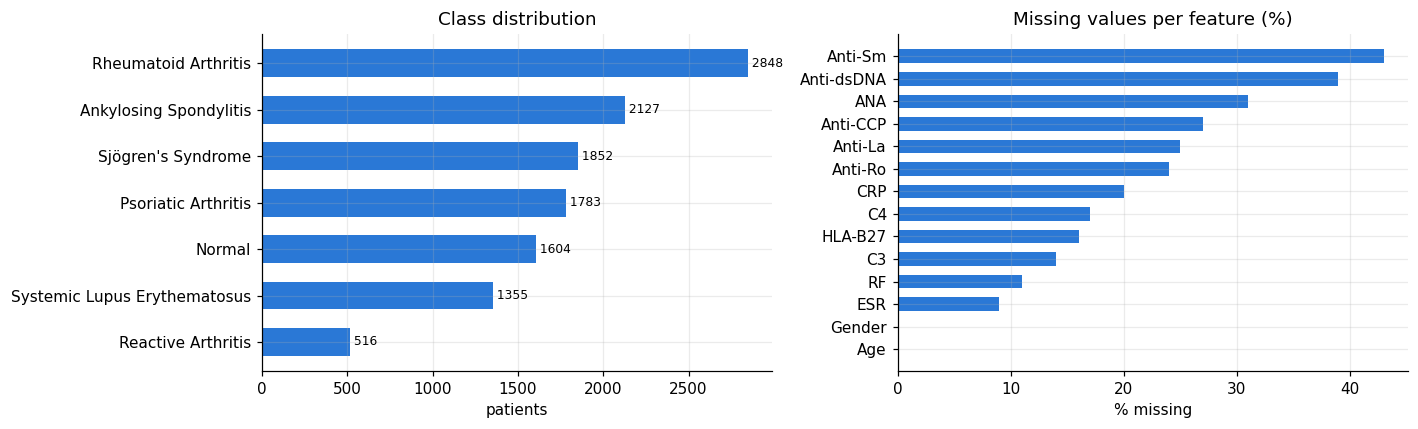
\includegraphics[width=0.85\textwidth]{figs/eda.png}
\caption{Rheumatic and autoimmune disease dataset~\cite{mahdi2025data}: class sizes (left) and percentage of missing values per variable before imputation (right).}
\label{fig:eda}
\end{figure*}

\subsection{Protocols}
\emph{Rheumatic data.} A single stratified 80/20 split (9,668 training and 2,417 test patients) was used for the main runs, so the ten seeds vary only the search. Binary variables were encoded as 0/1. Mean imputation and standardization for numeric variables, and mode imputation for binary variables, were fitted on the training split only. The fitness used the mean 3-fold stratified cross-validated accuracy of an XGBoost~\cite{chen2016xgb} and a histogram gradient-boosting classifier (60 trees, depth 4, learning rate 0.1), with SMOTE~\cite{chawla2002} applied inside each training fold. To keep the run time manageable, it was computed on a fixed stratified subsample of 4,000 training patients. For the final evaluation, both classifiers were retrained with 200 trees on the full training split, and we report their mean test accuracy and macro-F1. Each run had 12 agents and a budget of $B=252$ evaluations. Seed 42 was used during development and was excluded; the evaluation uses seeds 0--9.

\emph{Repeated clinical splits.} To check that the clinical results do not depend on one split, we drew two further stratified 80/20 splits (random states 1 and 2). On each, the imputation, the scaling and the 4,000-patient fitness subsample were refitted on that split's training data, and every method was run with seeds 0--4. Together with seeds 0--4 of the main runs this gives 3 splits $\times$ 5 seeds = 15 paired runs per method. We had planned four new splits and reduced them to two because of compute time (each new split needs about an hour of fresh fitness evaluations on the hardware we used); the reduction was decided before any of the new splits had finished.

\emph{Gene-expression and medical tabular data.} For each seed, a new stratified 70/30 split was drawn and min-max scaling was fitted on the training part. The fitness used the 5-fold cross-validated accuracy (balanced accuracy for GSE93272 and the tabular datasets) of a 5-nearest-neighbour classifier on the training part, and the test score is that of the same classifier retrained on the training part. For GSE93272, the 5,000 most variable probes were selected on each training split before the search. Each run had 20 agents and a budget of $B=1{,}020$ evaluations. The gene-expression runs used the sparse start and the tabular runs the dense start ($D<100$).

\emph{Second classifier.} After the main results, we repeated the tabular benchmark with a support vector machine (RBF kernel, $C=1$, $\gamma$ set by scikit-learn's \texttt{scale} rule, untuned) in place of 5-NN, in both the fitness and the test evaluation, with the same splits, seeds and budgets. Every wrapper and filter method, the two add-ons and PERTURB alone were rerun.

\subsection{Baselines}
All wrapper methods share the fitness function and the budget. The GA, binary PSO and binary GWO use the same initial population as the other methods. The GA uses tournament selection (size 3), uniform crossover (rate 0.9) and bit-flip mutation (rate $1/D$) with one elite. Binary PSO~\cite{kennedy1997} uses sigmoid velocity transfer, $c_1=c_2=2$, velocity clamp 6 and inertia decreasing from 0.9 to 0.4; with the sparse start, its initial velocities are set consistent with the initial masks. Binary GWO~\cite{mirjalili2014gwo,emary2016bgwo} updates continuous positions and binarizes them with the same rule as DO and HO. On the rheumatic data the GA, PSO, GWO and filter results of the main runs come from the earlier runs of this study, which used the same fitness, split, seeds and budget.

The three non-wrapper methods rank features on the same training data used by the fitness. LASSO uses the absolute coefficients of an L1-penalized logistic regression~\cite{tibshirani1996} on standardized data ($C=0.5$). mRMR~\cite{peng2005} uses mutual information minus mean absolute correlation with the already selected features, chosen greedily for up to 2,000 features, with the remainder ordered by relevance. ReliefF~\cite{kononenko1994} uses 500 sampled instances and 10 neighbours. For each ranking, the number of retained features $k$ is the one that minimizes the fitness (\ref{eq:fitness}), searched over all $k\le D$ when $D\le40$ and over $k\in\{5,10,20,50,100,200,500,1000,2000,D\}$ otherwise. No test data is used to choose $k$. The full feature set is included as a reference.

\subsection{Hypotheses fixed in advance}
Before running the main experiments we fixed four hypotheses and their tests:
\begin{itemize}
\item \textbf{H1}: RL-DOHO reaches lower fitness than the published DO.
\item \textbf{H2}: RL-DOHO against the published HO, with no direction predicted.
\item \textbf{H3}: at three times the budget, the UCB controller with the gain reward reaches lower fitness than random arm selection.
\item \textbf{H4}: on gene data, the sparse start gives RL-DOHO lower fitness than the dense start.
\end{itemize}
H1--H3 were tested on the clinical and gene-expression datasets and H4 on the five gene-expression datasets, each with a two-sided sign test over the paired runs.

After those results were known, and before running the extension experiments (the tabular datasets, the add-ons, the Q-learning controller, the $\kappa$ sweep and the repeated splits), we fixed four more:
\begin{itemize}
\item \textbf{H5}: at three times the budget, Q-learning against random arm selection, with no direction predicted.
\item \textbf{H6}: GA+SI reaches lower fitness than the GA, and HO+SI lower than HO (Holm-corrected over the two).
\item \textbf{H7}: the stagnation trigger $\kappa\in\{1,2,3,4\}$ has no effect on RL-DOHO's fitness (Friedman test).
\item \textbf{H8}: on the repeated clinical splits, RL-DOHO against each other method, with no direction predicted.
\end{itemize}
H5--H7 were tested on all eleven datasets. Before the SVM runs we fixed a ninth:
\begin{itemize}
\item \textbf{H9}: with an SVM, the tabular findings replicate: RL-DOHO beats DO (H9a); RL-DOHO against HO (H9b), the GA against RL-DOHO (H9c) and RL-DOHO against PERTURB alone (H9e) with no direction predicted; HO+SI beats HO, and GA+SI against the GA with no direction predicted (H9d).
\end{itemize}
All other settings of RL-DOHO ($\varepsilon$, the reward weights, the UCB constant, the number of flipped features, the tabu redraws) were carried over unchanged from the earlier version of this study and were not tuned.

\subsection{Statistical analysis}
Following Dem\v{s}ar~\cite{demsar2006}, we use nonparametric tests:
\begin{itemize}
\item \textbf{Within each dataset:} a Friedman test~\cite{friedman1937} compares all 11 methods over the 10 seeds. RL-DOHO is compared with each other method by a Wilcoxon signed-rank test~\cite{wilcoxon1945}, with zero differences split between the two sides and a Holm correction~\cite{holm1979} over the ten comparisons.
\item \textbf{Across datasets:} we pool the paired runs and apply a two-sided sign test to the wins and losses, Holm-corrected over the ten comparisons per metric. These pooled tests treat the runs as independent although runs on the same dataset share data, so the dataset-level analysis below, with one observation per dataset, is the conservative check.
\item \textbf{Dataset-level view:} methods are ranked by their mean on each dataset and compared with the Friedman test and the Nemenyi critical difference~\cite{nemenyi1963}. With eleven datasets and eleven methods the critical difference is 4.55 rank units.
\end{itemize}
Ablation comparisons report unadjusted sign-test $p$-values, as exploratory results. Differences smaller than $10^{-12}$ count as ties.

%% ======================================================================
\section{Results}\label{sec:results}

\subsection{Rheumatic and autoimmune disease data}
Table~\ref{tab:rheum} and Fig.~\ref{fig:rheumbox} summarize the clinical results.
\begin{itemize}
\item \textbf{Within the DO--HO family}, RL-DOHO had the lowest mean fitness: 0.1832, against 0.1838 for HO, 0.1857 for DOHO and 0.2280 for DO.
\item \textbf{Against DO}, RL-DOHO was better in all ten runs on fitness, test accuracy and macro-F1 (Holm $p=0.020$ each).
\item \textbf{Against HO} (5/2/3) and DOHO (8/0/2; unadjusted $p=0.020$, Holm $p=0.12$), the fitness differences were not significant after correction.
\item \textbf{The GA and binary PSO reached lower fitness} (0.1821 and 0.1828), and RL-DOHO ranked third of 11. The GA found the best subset seen in any run (fitness 0.18200, 10 features) in 7 of 10 runs, BPSO in 4, and RL-DOHO and BGWO in one each.
\item \textbf{Against the filters}, RL-DOHO's fitness was lower than LASSO's and ReliefF's in all ten runs (Holm $p=0.020$ each). On test accuracy, however, ReliefF (84.97\%) and LASSO (84.92\%) were ahead of RL-DOHO (84.33\%) in all ten runs (Holm $p=0.020$). With a fixed split, LASSO is deterministic here and ReliefF nearly so, so this paired test mostly reflects RL-DOHO's run-to-run variation.
\item \textbf{Test accuracy range}: apart from DO (79.99\%), all methods fall between 83.85\% and 84.97\%, a range of about 27 of the 2,417 test patients.
\end{itemize}

\begin{table*}[t]
\centering
\caption{Rheumatic and autoimmune disease data: mean $\pm$ standard deviation over ten seeds, at a budget of 252 fitness evaluations. CV and test accuracy and macro-F1 in \%. Ranks are averaged over seeds (1 = best). Best value per column in bold.}
\label{tab:rheum}
\footnotesize
\setlength{\tabcolsep}{5pt}
\begin{tabular}{@{}lccccccc@{}}
\toprule
Method & Fitness & CV acc. & Test acc. & Test macro-F1 & Features & Rank (fitness) & Rank (test acc.) \\
\midrule
\textbf{RL-DOHO} & 0.1832 $\pm$ 0.0013 & \textbf{82.38} & 84.33 $\pm$ 0.42 & 83.96 & 12.2 & 3.50 & 6.70 \\
DO & 0.2280 $\pm$ 0.0273 & 77.63 & 79.99 $\pm$ 3.08 & 79.66 & \textbf{9.1} & 10.95 & 10.95 \\
HO & 0.1838 $\pm$ 0.0013 & 82.34 & 84.29 $\pm$ 0.09 & 83.88 & 12.6 & 4.30 & 7.00 \\
DOHO & 0.1857 $\pm$ 0.0022 & 82.16 & 84.45 $\pm$ 0.30 & 84.01 & 12.7 & 6.75 & 5.75 \\
\midrule
GA & \textbf{0.1821} $\pm$ 0.0002 & 82.36 & 84.45 $\pm$ 0.35 & 83.86 & 10.4 & \textbf{1.60} & 5.50 \\
BPSO & 0.1828 $\pm$ 0.0010 & 82.33 & 84.54 $\pm$ 0.32 & 84.06 & 11.0 & 3.00 & 5.50 \\
BGWO & 0.1894 $\pm$ 0.0116 & 81.62 & 83.85 $\pm$ 1.30 & 83.28 & 10.4 & 6.60 & 6.90 \\
\midrule
LASSO & 0.1868 $\pm$ 0.0000 & 82.00 & 84.92 $\pm$ 0.00 & \textbf{84.81} & 12.0 & 7.80 & 2.10 \\
mRMR & 0.1848 $\pm$ 0.0021 & 82.19 & 84.51 $\pm$ 0.45 & 84.15 & 11.9 & 5.50 & 5.40 \\
ReliefF & 0.1854 $\pm$ 0.0012 & 82.10 & \textbf{84.97} $\pm$ 0.04 & 84.76 & 11.4 & 6.40 & \textbf{1.40} \\
All features & 0.1884 $\pm$ 0.0000 & 81.98 & 83.97 $\pm$ 0.00 & 83.50 & 14.0 & 9.60 & 8.80 \\
\bottomrule
\end{tabular}
\end{table*}

\begin{figure*}[t]
\centering
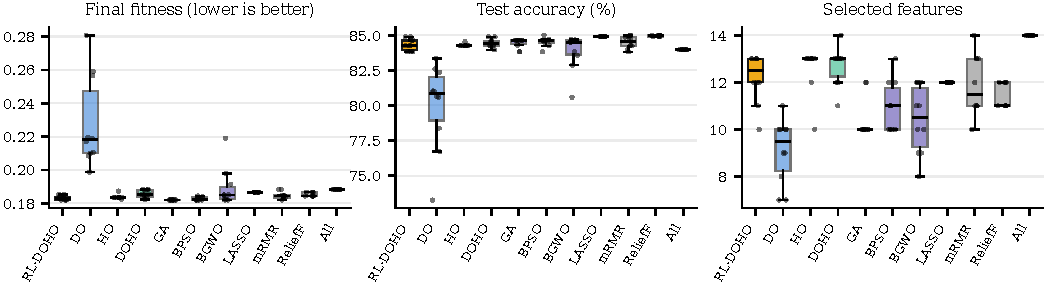
\includegraphics[width=\textwidth]{figs/rheum_box.pdf}
\caption{Rheumatic data: distribution over ten seeds of final fitness, test accuracy and subset size for every method (dots are individual runs; ``All'' is the full feature set).}
\label{fig:rheumbox}
\end{figure*}

Fig.~\ref{fig:convrheum} shows why DO fares so poorly on this problem. The published DO improved on the best subset of its initial population in only 1 of the 10 runs. Its landing stage places every agent close to the elite with small Lévy steps, so after the first iteration hardly any coordinate crosses zero and the population keeps producing the elite's subset. HO's greedy, randomized phases do not have this problem, and RL-DOHO escapes it through its interventions. On this dataset its DO exploration steps never lowered the best fitness, and 80\% of its total improvement came from the HO arm (Table~\ref{tab:arms}).

\begin{figure}[t]
\centering
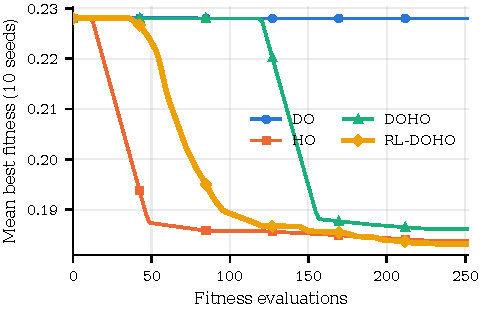
\includegraphics[width=\columnwidth]{figs/conv_rheum.pdf}
\caption{Mean best fitness against fitness evaluations used, over ten seeds, on the rheumatic data for the DO--HO family.}
\label{fig:convrheum}
\end{figure}

The selected variables were similar across the wrapper methods (Fig.~\ref{fig:freq}). RL-DOHO kept ESR, CRP, RF, anti-CCP, C3, C4, gender, ANA, anti-Ro and anti-La in every run and HLA-B27 in nine. It kept anti-dsDNA in two runs and anti-Sm in three: these are the two variables with the most missing values. The GA, which reached the lowest fitness, also dropped anti-dsDNA and anti-Sm and, unlike RL-DOHO, usually dropped age and HLA-B27. LASSO and ReliefF kept HLA-B27, anti-dsDNA (LASSO) and anti-Sm, and dropped age and gender.

\begin{figure}[t]
\centering
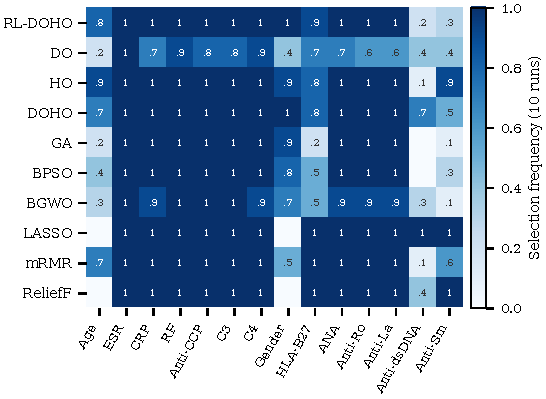
\includegraphics[width=\columnwidth]{figs/feat_freq.pdf}
\caption{Rheumatic data: fraction of the ten runs in which each method selected each variable (blank = never).}
\label{fig:freq}
\end{figure}

This comparison uses a single train/test split. Section~\ref{sec:splits} repeats it on two further splits.

\subsection{Gene-expression data}
Table~\ref{tab:genes} and Fig.~\ref{fig:convgenes} give the results on the five gene-expression datasets.
\begin{itemize}
\item \textbf{Against DO}, RL-DOHO reached lower fitness on all five datasets; the per-dataset difference was significant after correction on Colon, ALL/AML and Lung.
\item \textbf{Against HO}, its mean fitness was lower on Colon, ALL/AML and Glioma and higher on Lung and GSE93272, with no significant per-dataset difference; on ALL/AML HO was ahead in more runs (5 against 4).
\item \textbf{The GA} had the lowest wrapper fitness on four of the five datasets; RL-DOHO had it on ALL/AML.
\item \textbf{Binary PSO and GWO} kept many more genes than the other wrappers (240--1,280 on average, against 40--330), probably because their position updates drift away from the sparse initial masks.
\end{itemize}

\begin{table*}[t]
\centering
\caption{Gene-expression datasets: mean fitness, mean test accuracy (\%, balanced accuracy for GSE93272) and mean number of selected features ($|S|$) over ten seeds, each with its own train/test split, at a budget of 1,020 fitness evaluations. All wrapper methods start from the sparse initial population. Best value per column in bold.}
\label{tab:genes}
\footnotesize
\setlength{\tabcolsep}{3.2pt}
\begin{tabular}{@{}l ccc ccc ccc ccc ccc@{}}
\toprule
& \multicolumn{3}{c}{Colon} & \multicolumn{3}{c}{ALL/AML} & \multicolumn{3}{c}{Lung} & \multicolumn{3}{c}{Glioma} & \multicolumn{3}{c}{GSE93272} \\
\cmidrule(lr){2-4}\cmidrule(lr){5-7}\cmidrule(lr){8-10}\cmidrule(lr){11-13}\cmidrule(l){14-16}
Method & Fit. & Acc. & $|S|$ & Fit. & Acc. & $|S|$ & Fit. & Acc. & $|S|$ & Fit. & Acc. & $|S|$ & Fit. & Acc. & $|S|$ \\
\midrule
\textbf{RL-DOHO} & 0.083 & 73.7 & 58 & 0.052 & 83.2 & 63 & 0.034 & 93.3 & 231 & 0.145 & 78.7 & 333 & 0.079 & 87.1 & 100 \\
DO & 0.127 & 71.1 & 70 & 0.105 & 80.5 & 115 & 0.045 & 94.4 & 217 & 0.184 & 75.3 & 69 & 0.095 & 84.9 & 148 \\
HO & 0.090 & 71.1 & 63 & 0.059 & 80.0 & 43 & 0.033 & 93.3 & 241 & 0.153 & 76.7 & 63 & 0.073 & 88.1 & 82 \\
DOHO & 0.111 & 71.1 & 64 & 0.079 & 80.9 & 61 & 0.036 & 93.8 & 226 & 0.170 & 78.7 & 85 & 0.087 & 85.8 & 142 \\
\midrule
GA & 0.062 & 76.3 & 62 & 0.054 & 83.6 & 150 & 0.028 & 93.3 & 162 & 0.111 & 76.7 & 91 & 0.053 & 87.4 & 141 \\
BPSO & 0.137 & 73.7 & 239 & 0.112 & 82.3 & 950 & 0.037 & 94.4 & 590 & 0.197 & 80.0 & 628 & 0.113 & 87.4 & 941 \\
BGWO & 0.100 & 75.3 & 390 & 0.093 & 82.7 & 1278 & 0.034 & 93.6 & 611 & 0.188 & 81.3 & 558 & 0.092 & 86.5 & 1025 \\
\midrule
LASSO & \textbf{0.028} & \textbf{82.1} & \textbf{16} & \textbf{0.008} & 91.4 & \textbf{33} & \textbf{0.019} & 94.4 & \textbf{77} & \textbf{0.009} & 67.3 & \textbf{18} & \textbf{0.004} & 88.9 & \textbf{48} \\
mRMR & 0.104 & 80.0 & 83 & 0.012 & \textbf{94.1} & 110 & 0.024 & \textbf{95.1} & 170 & 0.119 & 77.3 & 86 & 0.061 & \textbf{89.4} & 182 \\
ReliefF & 0.093 & 77.9 & 41 & 0.036 & 92.7 & 57 & 0.044 & 93.6 & 645 & 0.150 & 75.3 & 64 & 0.093 & 82.8 & 115 \\
All features & 0.260 & 72.6 & 2000 & 0.212 & 82.3 & 7129 & 0.067 & 94.3 & 3312 & 0.299 & \textbf{84.0} & 4434 & 0.191 & 85.3 & 5000 \\
\bottomrule
\end{tabular}
\end{table*}

\begin{figure*}[t]
\centering
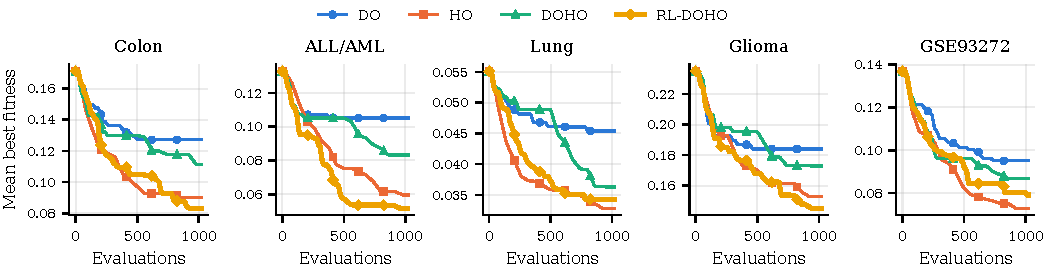
\includegraphics[width=\textwidth]{figs/conv_genes.pdf}
\caption{Mean best fitness against fitness evaluations, over ten seeds, on the gene-expression datasets for the DO--HO family (20 agents, 1,020 evaluations).}
\label{fig:convgenes}
\end{figure*}

The filter methods behaved as in earlier work. LASSO reached the lowest fitness on every dataset, using 16--77 genes on average. mRMR had lower mean fitness than RL-DOHO on four of the five datasets, significantly so on ALL/AML and Lung. RL-DOHO reached lower fitness than ReliefF on Lung (Holm $p=0.035$). On held-out data the picture changes:
\begin{itemize}
\item Only two per-dataset test-accuracy differences between RL-DOHO and a filter were significant: mRMR and ReliefF were ahead on ALL/AML (Holm $p=0.039$).
\item On Glioma, LASSO had the best fitness (0.0085) but the lowest test accuracy (67.3\% against 78.7\% for RL-DOHO). RL-DOHO's macro-F1 was higher in all ten runs (Holm $p=0.020$).
\item With 15--61 test samples per split, one sample is worth 1.6--6.7 accuracy points, so these test accuracies are coarse.
\end{itemize}
Fig.~\ref{fig:size} plots test accuracy against subset size.

\begin{figure*}[t]
\centering
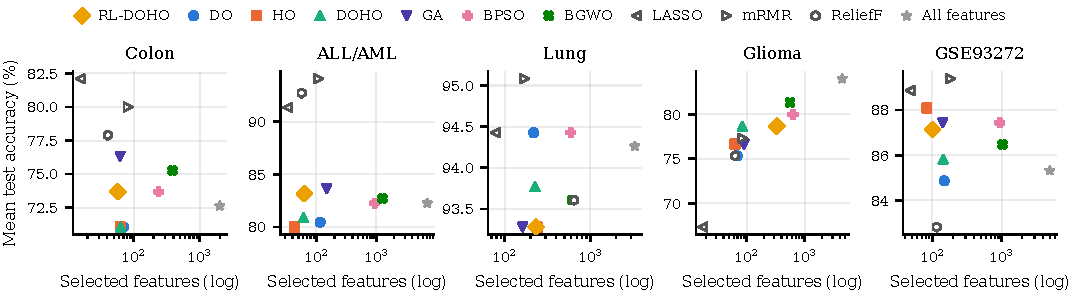
\includegraphics[width=\textwidth]{figs/acc_vs_size.pdf}
\caption{Mean test accuracy against mean number of selected features (log scale) on the gene-expression datasets. Hollow markers are filter or embedded methods.}
\label{fig:size}
\end{figure*}


\subsection{Medical tabular datasets}
Table~\ref{tab:tab} gives the results on the five medical tabular datasets.
\begin{itemize}
\item \textbf{Against DO}, RL-DOHO reached lower fitness in 49 of 50 runs, significantly so on every dataset after correction.
\item \textbf{Against HO} it was ahead in 30 runs and behind in 20 (Holm $p=0.61$), with no significant per-dataset difference; against the fixed hybrid it was ahead in 35 and behind in 15 (Holm $p=0.026$).
\item \textbf{The GA} reached lower fitness than RL-DOHO in 45 of the 50 runs and on every dataset, significantly so on four of the five. Binary PSO and GWO were level with RL-DOHO (each ahead in 30 runs and behind in 20, Holm $p=0.61$).
\item \textbf{Against the filters}, RL-DOHO reached lower fitness than mRMR and ReliefF in 48 of 50 runs and than LASSO in 38 (all Holm $p\le0.002$). Unlike on gene data, the filters did not lead on fitness here.
\item \textbf{Test scores:} the per-dataset Friedman test on test balanced accuracy was not significant on any of the five datasets ($p=0.21$--$0.97$), and no pooled test-accuracy or macro-F1 comparison was significant after correction.
\item \textbf{Two datasets are hard for 5-NN.} Averaged over the 11 methods, test balanced accuracy was 53.6\% on Backache and 63.7\% on Hepatitis, and their test sets hold only about 8 and 10 minority-class patients. Fitness differences there say little about held-out performance, so Section~\ref{sec:pooled} checks which conclusions depend on these two datasets.
\end{itemize}
Over the 50 tabular runs RL-DOHO had an average per-run fitness rank of 4.15 among the 11 methods, behind the GA (1.82), binary PSO (3.28) and binary GWO (3.29), and ahead of HO (4.75).

\begin{table*}[t]
\centering
\caption{Medical tabular datasets: mean fitness, mean test balanced accuracy (\%) and mean number of selected features ($|S|$) over ten seeds, each with its own train/test split, at a budget of 1,020 fitness evaluations. All wrapper methods start from the dense initial population. Best value per column in bold.}
\label{tab:tab}
\footnotesize
\setlength{\tabcolsep}{3.2pt}
\begin{tabular}{@{}l ccc ccc ccc ccc ccc@{}}
\toprule
& \multicolumn{3}{c}{WDBC} & \multicolumn{3}{c}{Hepatitis} & \multicolumn{3}{c}{Dermatology} & \multicolumn{3}{c}{SPECTF} & \multicolumn{3}{c}{Backache} \\
\cmidrule(lr){2-4}\cmidrule(lr){5-7}\cmidrule(lr){8-10}\cmidrule(lr){11-13}\cmidrule(l){14-16}
Method & Fit. & Acc. & $|S|$ & Fit. & Acc. & $|S|$ & Fit. & Acc. & $|S|$ & Fit. & Acc. & $|S|$ & Fit. & Acc. & $|S|$ \\
\midrule
\textbf{RL-DOHO} & 0.029 & 94.3 & 13 & 0.209 & 64.2 & \textbf{7} & 0.025 & 95.0 & 17 & 0.167 & 73.1 & 22 & 0.316 & 54.3 & 10 \\
DO & 0.041 & 94.2 & 16 & 0.269 & 64.6 & 9 & 0.050 & 94.3 & 18 & 0.225 & 73.8 & 23 & 0.388 & 53.3 & 17 \\
HO & 0.032 & 94.5 & 13 & 0.221 & 62.1 & 7 & 0.026 & 95.4 & 24 & 0.178 & 73.7 & 18 & 0.310 & 53.8 & 12 \\
DOHO & 0.034 & 94.6 & 14 & 0.219 & 63.4 & 7 & 0.030 & 96.0 & 25 & 0.190 & 71.1 & 19 & 0.325 & 54.3 & 13 \\
\midrule
GA & \textbf{0.025} & 94.7 & 14 & 0.198 & 66.3 & 8 & \textbf{0.016} & 95.6 & \textbf{16} & \textbf{0.131} & 75.3 & 21 & \textbf{0.284} & 54.2 & 12 \\
BPSO & 0.029 & 95.2 & 15 & \textbf{0.189} & 61.7 & 8 & 0.020 & 95.2 & 20 & 0.172 & \textbf{75.8} & 22 & 0.297 & 52.6 & 14 \\
BGWO & 0.028 & 94.5 & 14 & 0.221 & \textbf{66.4} & 8 & 0.019 & 95.8 & 19 & 0.156 & 75.5 & 24 & 0.300 & 53.7 & 13 \\
\midrule
LASSO & 0.033 & 94.8 & \textbf{11} & 0.249 & 63.6 & 9 & 0.026 & 96.0 & 18 & 0.214 & 73.1 & \textbf{11} & 0.367 & 53.1 & \textbf{9} \\
mRMR & 0.036 & 94.5 & 13 & 0.251 & 62.4 & 8 & 0.039 & \textbf{96.1} & 23 & 0.285 & 68.9 & 23 & 0.382 & 53.4 & 14 \\
ReliefF & 0.036 & 94.0 & 12 & 0.264 & 59.9 & 8 & 0.039 & 95.7 & 30 & 0.238 & 74.3 & 15 & 0.387 & 52.7 & 13 \\
All features & 0.053 & \textbf{95.3} & 30 & 0.323 & 65.7 & 19 & 0.059 & 95.2 & 34 & 0.314 & 70.7 & 44 & 0.433 & \textbf{54.4} & 32 \\
\bottomrule
\end{tabular}
\end{table*}

\subsection{Comparison across all eleven datasets}\label{sec:pooled}
Table~\ref{tab:pooled} pools the 110 paired runs.
\begin{itemize}
\item \textbf{Fitness, against the other wrapper methods:} RL-DOHO was ahead of DO in 103 runs and behind in 4, ahead of DOHO in 81 and behind in 28, and ahead of binary PSO in 70 and behind in 38. All three differences are significant after correction. Against binary GWO it was ahead in 67 runs and behind in 43 (Holm $p=0.084$).
\item \textbf{Against HO}, it was level (58 against 49, Holm $p=0.59$).
\item \textbf{The GA} reached lower fitness significantly more often (85 against 22, Holm $p<0.001$).
\item \textbf{Against the filters}, RL-DOHO was ahead of ReliefF (84 against 26) and mRMR (68 against 40) after correction and level with LASSO (49 against 61), which led on gene data and trailed on the other two data types.
\item \textbf{Test accuracy:} no comparison was significant after correction. On macro-F1, LASSO was ahead of RL-DOHO (66 against 36, Holm $p=0.039$).
\end{itemize}
Restricted to the six datasets of the main study (60 runs), the figures are those of the earlier analysis: ahead of DO 54 against 3, level with HO 28 against 29, behind the GA 18 against 40.

\emph{Sensitivity to the two weakest datasets.} Table~\ref{tab:weak} repeats the main comparisons without Backache and Hepatitis (90 runs). The conclusions about DO, HO, the GA, the fixed hybrid, binary PSO, the add-ons, the controllers and $\kappa$ are unchanged. One result does not survive: RL-DOHO's lead over mRMR (48 against 40, $p=0.46$). The advantage of PERTURB alone over the full arm set also becomes non-significant over the remaining 90 runs (47 against 37, $p=0.33$), but only because those runs are dominated by the gene data, where PERTURB alone is behind; on the three remaining tabular datasets it is still ahead (22 against 5, $p=0.002$).

\begin{table}[t]
\centering
\caption{Main comparisons with and without the two weakest datasets (Backache and Hepatitis): W/T/L for the first-named method on fitness and unadjusted two-sided sign-test $p$.}
\label{tab:weak}
\footnotesize
\setlength{\tabcolsep}{2.4pt}
\begin{tabular}{@{}lcccc@{}}
\toprule
& \multicolumn{2}{c}{All 11 datasets} & \multicolumn{2}{c}{Without the two} \\
\cmidrule(lr){2-3}\cmidrule(l){4-5}
Comparison & W/T/L & $p$ & W/T/L & $p$ \\
\midrule
RL-DOHO vs.\ DO & 103/3/4 & $<$0.001 & 83/3/4 & $<$0.001 \\
RL-DOHO vs.\ HO & 58/3/49 & 0.439 & 47/3/40 & 0.520 \\
RL-DOHO vs.\ DOHO & 81/1/28 & $<$0.001 & 69/1/20 & $<$0.001 \\
RL-DOHO vs.\ GA & 22/3/85 & $<$0.001 & 19/2/69 & $<$0.001 \\
RL-DOHO vs.\ BPSO & 70/2/38 & 0.003 & 64/2/24 & $<$0.001 \\
RL-DOHO vs.\ mRMR & 68/2/40 & 0.009 & 48/2/40 & 0.456 \\
HO+SI vs.\ HO & 71/10/29 & $<$0.001 & 54/8/28 & 0.005 \\
GA+SI vs.\ GA & 45/16/49 & 0.757 & 36/10/44 & 0.434 \\
PERTURB only vs.\ RL-DOHO & 64/6/40 & 0.024 & 47/6/37 & 0.326 \\
Q-learning vs.\ random arm, 3$\times$ & 46/8/56 & 0.373 & 37/7/46 & 0.380 \\
$\kappa\in\{1,2,3,4\}$ (Friedman) & -- & $<$0.001 & -- & $<$0.001 \\
\bottomrule
\end{tabular}
\end{table}

\begin{table}[t]
\centering
\caption{RL-DOHO against each method over all 110 paired runs (11 datasets $\times$ 10 seeds): wins/ties/losses for RL-DOHO and Holm-adjusted sign-test $p$-values. Bold: $p<0.05$.}
\label{tab:pooled}
\footnotesize
\setlength{\tabcolsep}{2.6pt}
\begin{tabular}{@{}lcccccc@{}}
\toprule
& \multicolumn{2}{c}{Fitness} & \multicolumn{2}{c}{Test accuracy} & \multicolumn{2}{c}{Macro-F1} \\
\cmidrule(lr){2-3}\cmidrule(lr){4-5}\cmidrule(l){6-7}
vs. & W/T/L & $p$ & W/T/L & $p$ & W/T/L & $p$ \\
\midrule
DO & 103/3/4 & \textbf{$<$0.001} & 58/14/38 & 0.467 & 57/8/45 & 1.000 \\
HO & 58/3/49 & 0.588 & 52/12/46 & 1.000 & 55/7/48 & 1.000 \\
DOHO & 81/1/28 & \textbf{$<$0.001} & 44/13/53 & 1.000 & 47/7/56 & 1.000 \\
\midrule
GA & 22/3/85 & \textbf{$<$0.001} & 48/14/48 & 1.000 & 52/11/47 & 1.000 \\
BPSO & 70/2/38 & \textbf{0.013} & 49/14/47 & 1.000 & 51/10/49 & 1.000 \\
BGWO & 67/0/43 & 0.084 & 43/12/55 & 1.000 & 44/7/59 & 1.000 \\
\midrule
LASSO & 49/0/61 & 0.588 & 36/11/63 & 0.086 & 36/8/66 & \textbf{0.039} \\
mRMR & 68/2/40 & \textbf{0.036} & 41/11/58 & 0.751 & 42/9/59 & 0.887 \\
ReliefF & 84/0/26 & \textbf{$<$0.001} & 41/10/59 & 0.709 & 42/7/61 & 0.681 \\
All features & 110/0/0 & \textbf{$<$0.001} & 44/14/52 & 1.000 & 45/10/55 & 1.000 \\
\bottomrule
\end{tabular}
\end{table}

Fig.~\ref{fig:cd} ranks the methods by their mean on each dataset.
\begin{itemize}
\item \textbf{Fitness:} the dataset-level Friedman test is significant ($\chi^2=62.99$, $p<0.001$). The GA (1.91) ranks first and RL-DOHO second (4.00), followed by LASSO (4.18), HO (4.82), BGWO (5.36), BPSO (5.73), mRMR (5.91), DOHO (6.55), ReliefF (7.27), DO (9.45) and the full feature set (10.82). Thirteen pairs exceed the critical difference. RL-DOHO is separated from DO and from the full feature set, and the GA additionally from DOHO and ReliefF; RL-DOHO is not separated from the GA or from HO.
\item \textbf{Test accuracy:} the dataset-level Friedman test is not significant ($\chi^2=16.23$, $p=0.093$), and no pair exceeds the critical difference.
\end{itemize}

\begin{figure*}[t]
\centering
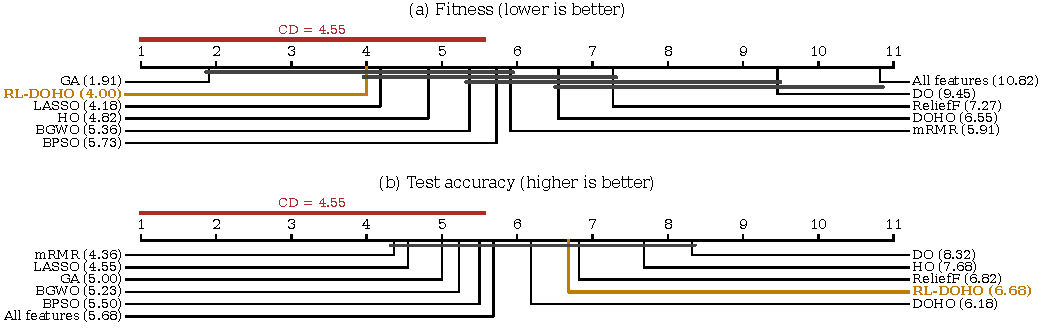
\includegraphics[width=0.92\textwidth]{figs/cd.pdf}
\caption{Critical-difference diagrams over the eleven datasets (methods ranked by their mean on each dataset; Nemenyi test, $\alpha=0.05$, CD $=4.55$). Thick bars join methods whose average ranks differ by less than the critical difference. Labels are split between the two sides for readability: a method's rank is given by where its line meets the axis (further left is better), not by its label's side or vertical position.}
\label{fig:cd}
\end{figure*}

\subsection{Consistency within the DO--HO family}
Table~\ref{tab:family} ranks the four family members against each other in every run.
\begin{itemize}
\item The family-only Friedman test is significant on all eleven datasets, mostly because DO trails the others.
\item RL-DOHO had the best average rank (1.77), ahead of HO (1.89), DOHO (2.63) and DO (3.72). It was the best or tied best of the four in 50\% of runs, against 40\% for HO.
\item RL-DOHO was the worst of the four in only 2 of the 110 runs (HO: 5\%, DOHO: 16\%, DO: 85\% of runs, ties included).
\item Averaged over all 110 runs, RL-DOHO's fitness was 0.0082 above the run's best family member, against 0.0114 for HO. Its single largest gap (0.120, on Glioma) was larger than HO's (0.085).
\end{itemize}
RL-DOHO and HO did not differ significantly in a direct comparison (58 against 49), and on the repeated clinical splits HO had the better family rank (Section~\ref{sec:splits}), so the family ranking shows consistency rather than a clear winner.

\begin{table}[t]
\centering
\caption{Average per-run rank on fitness within the DO--HO family (1 = best of four), family-only Friedman $p$-value per dataset, and how often each method was the best or the worst of the four over the 110 runs (ties counted for every tied method).}
\label{tab:family}
\footnotesize
\setlength{\tabcolsep}{3.5pt}
\begin{tabular}{@{}lccccc@{}}
\toprule
Dataset & RL-DOHO & DO & HO & DOHO & Friedman $p$ \\
\midrule
Rheumatic & \textbf{1.60} & 4.00 & 1.85 & 2.55 & $<$0.001 \\
\midrule
Colon & \textbf{1.75} & 3.45 & 1.90 & 2.90 & 0.007 \\
ALL/AML & \textbf{1.70} & 3.60 & 1.75 & 2.95 & 0.001 \\
Lung & 2.10 & 3.80 & \textbf{1.70} & 2.40 & 0.002 \\
Glioma & \textbf{1.50} & 3.25 & 2.30 & 2.95 & 0.011 \\
GSE93272 & 2.20 & 3.20 & \textbf{1.50} & 3.10 & 0.009 \\
\midrule
WDBC & \textbf{1.50} & 3.85 & 2.30 & 2.35 & $<$0.001 \\
Hepatitis & \textbf{1.80} & 3.95 & 2.05 & 2.20 & $<$0.001 \\
Dermatology & 1.90 & 3.85 & \textbf{1.70} & 2.55 & $<$0.001 \\
SPECTF & \textbf{1.50} & 3.95 & 2.00 & 2.55 & $<$0.001 \\
Backache & 1.90 & 4.00 & \textbf{1.70} & 2.40 & $<$0.001 \\
\midrule
Mean (110 runs) & \textbf{1.77} & 3.72 & 1.89 & 2.63 & -- \\
Best or tied (\%) & \textbf{50} & 3 & 40 & 15 & -- \\
Worst or tied (\%) & \textbf{2} & 85 & 5 & 16 & -- \\
\bottomrule
\end{tabular}
\end{table}

\subsection{Hypotheses H1--H8}
Table~\ref{tab:hyp} reports the eight hypotheses fixed in advance.
\begin{itemize}
\item \textbf{H1} was supported, and the tabular datasets replicate it (49 against 1).
\item \textbf{H2} showed no difference, and the tabular datasets agree (30 against 20, $p=0.20$).
\item \textbf{H3} was not supported: at three times the budget, the bandit and random arm selection reached lower fitness about equally often (27 against 29). On the tabular data the bandit was ahead in 28 runs and random selection in 20 ($p=0.31$).
\item \textbf{H4} was supported.
\item \textbf{H5} showed no difference between Q-learning and random selection (46 against 56).
\item \textbf{H6} was half supported: the intervention layer improved HO but not the GA (Section~\ref{sec:addon}).
\item \textbf{H7} was rejected: $\kappa$ affects fitness (Section~\ref{sec:kappa}).
\item \textbf{H8} found significant differences only against DO and the full feature set (Section~\ref{sec:splits}).
\item \textbf{H9}: every tested tabular finding replicated with an SVM, including the advantage of PERTURB alone (Section~\ref{sec:svm}).
\end{itemize}

\begin{table}[t]
\centering
\caption{Hypotheses fixed in advance: W/T/L for the first-named method and two-sided sign-test $p$ (H6: Holm-corrected over the two comparisons; H7: Friedman test over the four values of $\kappa$; H8: summary of twelve Holm-corrected comparisons; H9: tabular data with an SVM).}
\label{tab:hyp}
\footnotesize
\setlength{\tabcolsep}{2.0pt}
\begin{tabular}{@{}llccl@{}}
\toprule
& Comparison (fitness) & Runs & W/T/L & $p$ \\
\midrule
H1 & RL-DOHO vs.\ published DO & 60 & 54/3/3 & $<$0.001 \\
H2 & RL-DOHO vs.\ published HO & 60 & 28/3/29 & 1.000 \\
H3 & UCB (gain) vs.\ random, 3$\times$ budget & 60 & 27/4/29 & 0.894 \\
H4 & Sparse vs.\ dense start (gene data) & 50 & 46/0/4 & $<$0.001 \\
\midrule
H5 & Q-learning vs.\ random, 3$\times$ budget & 110 & 46/8/56 & 0.373 \\
H6 & GA+SI vs.\ GA & 110 & 45/16/49 & 0.757 \\
   & HO+SI vs.\ HO & 110 & 71/10/29 & $<$0.001 \\
H7 & $\kappa\in\{1,2,3,4\}$ (Friedman) & 110 & -- & $<$0.001 \\
H8 & RL-DOHO vs.\ each, repeated splits & 15 & see Table~\ref{tab:splits} & -- \\
\midrule
H9a & RL-DOHO vs.\ DO (SVM) & 50 & 50/0/0 & $<$0.001 \\
H9b & RL-DOHO vs.\ HO (SVM) & 50 & 32/0/18 & 0.065 \\
H9c & GA vs.\ RL-DOHO (SVM) & 50 & 43/2/5 & $<$0.001 \\
H9d & HO+SI vs.\ HO (SVM) & 50 & 37/5/8 & $<$0.001 \\
 & GA+SI vs.\ GA (SVM) & 50 & 16/17/17 & 1.000 \\
H9e & RL-DOHO vs.\ PERTURB alone (SVM) & 50 & 8/1/41 & $<$0.001 \\
\bottomrule
\end{tabular}
\end{table}

\subsection{Ablation and controllers}\label{sec:ablation}
Table~\ref{tab:ablation} and Fig.~\ref{fig:abl} vary one component at a time.
\begin{itemize}
\item \textbf{The interventions:} removing them leaves essentially the published DO (run inside the RL-DOHO loop). That made results worse in 103 of the 110 runs ($p<0.001$), on every data type.
\item \textbf{The sparse start:} replacing it with the dense start was worse in 46 of 50 gene runs ($p<0.001$), with mean fitness 0.1269 against 0.0786 and about 870 genes against 157.
\item \textbf{The controller:} random arm selection was level with the bandit on every data type (54 against 51 overall). The Q-learning controller was behind the bandit in 62 runs and ahead in 45 ($p=0.12$); its deficit was largest on the clinical data (8 against 1, $p=0.039$) and absent on the tabular data (23 against 27). It was also level with random selection (44 against 62, $p=0.098$). The old reward gave the same results in 7 of 10 clinical runs and was level on gene data.
\item \textbf{PERTURB alone} was ahead of the full arm set on the clinical (6 against 2) and tabular data (39 against 8, $p<0.001$), and behind it on gene data (19 against 30, $p=0.15$). Over all 110 runs it was ahead in 64 and behind in 40 ($p=0.024$, unadjusted). The advantage is specific to the low-dimensional data, and it replicated with an SVM (Section~\ref{sec:svm}).
\item \textbf{The parsimony tie-break} changed no clinical run.
\item \textbf{At three times the budget}, the controllers ended level on every data type (Table~\ref{tab:ablation}, bottom). On the clinical data all three reached a mean fitness of about 0.1824 with about 10.4 features, close to the best subset found by any run (0.1820, 10 features).
\end{itemize}

\begin{table*}[t]
\centering
\caption{Ablation and controllers. Top: at the standard budget, mean fitness and W/T/L of the full method (UCB1, gain reward) against each variant. Bottom: the controllers at three times the budget. Sign-test $p$ unadjusted. The old reward, the tie-break and the dense start were run in the earlier part of the study only (the dense start applies to gene data only).}
\label{tab:ablation}
\footnotesize
\setlength{\tabcolsep}{3.4pt}
\begin{tabular}{@{}lccccccc@{}}
\toprule
& \multicolumn{2}{c}{Clinical (10 runs)} & \multicolumn{2}{c}{Gene expression (50)} & \multicolumn{2}{c}{Medical tabular (50)} & All (110) \\
\cmidrule(lr){2-3}\cmidrule(lr){4-5}\cmidrule(lr){6-7}\cmidrule(l){8-8}
Variant & Fitness & W/T/L ($p$) & Fitness & W/T/L ($p$) & Fitness & W/T/L ($p$) & W/T/L ($p$) \\
\midrule
RL-DOHO (UCB1, gain reward) & 0.1832 & -- & 0.0786 & -- & 0.1494 & -- & -- \\
Q-learning controller & 0.1846 & 8/1/1 (0.039) & 0.0853 & 31/2/17 (0.059) & 0.1507 & 23/0/27 (0.672) & 62/3/45 (0.122) \\
Random arm & 0.1846 & 6/2/2 (0.289) & 0.0815 & 25/2/23 (0.885) & 0.1487 & 23/1/26 (0.775) & 54/5/51 (0.845) \\
PERTURB only & 0.1825 & 2/2/6 (0.289) & 0.0860 & 30/1/19 (0.152) & 0.1359 & 8/3/39 ($<$0.001) & 40/6/64 (0.024) \\
UCB1, old reward & 0.1836 & 2/7/1 (1.000) & 0.0828 & 23/7/20 (0.761) & -- & -- & -- \\
No tie-break & 0.1832 & 0/10/0 (1.000) & -- & -- & -- & -- & -- \\
Dense start & -- & -- & 0.1269 & 46/0/4 ($<$0.001) & -- & -- & -- \\
No intervention (DO) & 0.2280 & 10/0/0 (0.002) & 0.1113 & 44/3/3 ($<$0.001) & 0.1946 & 49/0/1 ($<$0.001) & 103/3/4 ($<$0.001) \\
\midrule
\multicolumn{8}{@{}l@{}}{\emph{Three times the budget (756 and 3,060 evaluations): UCB1 with the gain reward against each alternative}} \\
\midrule
UCB1, gain reward & 0.1824 & -- & 0.0676 & -- & 0.1372 & -- & -- \\
Q-learning & 0.1824 & 1/4/5 (0.219) & 0.0703 & 29/1/20 (0.253) & 0.1371 & 25/1/24 (1.000) & 55/6/49 (0.624) \\
Random arm & 0.1824 & 4/3/3 (1.000) & 0.0645 & 23/1/26 (0.775) & 0.1379 & 28/2/20 (0.312) & 55/6/49 (0.624) \\
UCB1, old reward & 0.1825 & 3/3/4 (1.000) & 0.0686 & 21/3/26 (0.560) & -- & -- & -- \\
\bottomrule
\end{tabular}
\end{table*}



\begin{figure*}[t]
\centering
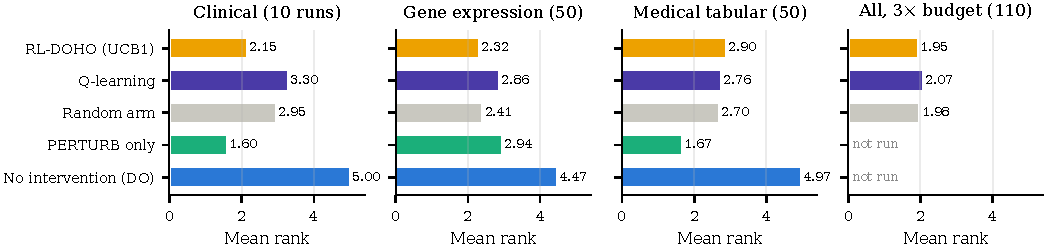
\includegraphics[width=\textwidth]{figs/ablation.pdf}
\caption{Mean per-run fitness rank of the controller variants within each group of runs (lower is better). ``No intervention'' is the published DO; it was not run at three times the budget.}
\label{fig:abl}
\end{figure*}
\subsection{What the controller did}
Table~\ref{tab:arms} and Fig.~\ref{fig:trace} show how the controller was used in the main runs.
\begin{itemize}
\item \textbf{Clinical runs:} the bandit made 9.4 decisions per run, four of them the initial pull of each arm. Its reward-driven choices favoured PERTURB (35\%) and HO (31\%), the two arms that ever lowered the best fitness.
\item \textbf{Gene runs:} it made 27.3 decisions per run, and its choices stayed close to uniform. DO exploration steps produced 42\% of the total fitness reduction, PERTURB 26\% and the HO arm 21\%.
\end{itemize}
Different arms carried the search on different problems, yet a random choice among them performed as well as the learned one.

\begin{table}[t]
\centering
\caption{Controller behaviour in the main RL-DOHO runs (10 clinical runs; 50 gene-expression runs over five datasets).}
\label{tab:arms}
\footnotesize
\setlength{\tabcolsep}{5pt}
\begin{tabular}{@{}lcc@{}}
\toprule
& Clinical & Gene expression \\
\midrule
Controller decisions per run & 9.4 & 27.3 \\
\quad of which initial (one per arm) & 4.0 & 4.0 \\
\midrule \multicolumn{3}{l}{\emph{Share of UCB-driven choices (\%)}} \\
\quad PERTURB & 35 & 26 \\
\quad RESTART & 17 & 21 \\
\quad DO & 17 & 28 \\
\quad HO & 31 & 25 \\
\midrule \multicolumn{3}{l}{\emph{Pulls that lowered the best fitness (\%)}} \\
\quad PERTURB & 45 & 16 \\
\quad RESTART & 0 & 2 \\
\quad DO & 0 & 8 \\
\quad HO & 48 & 34 \\
\midrule \multicolumn{3}{l}{\emph{Share of total fitness reduction (\%)}} \\
\quad DO exploration steps & 0.0 & 41.9 \\
\quad PERTURB & 19.5 & 25.6 \\
\quad RESTART & 0.0 & 2.9 \\
\quad DO arm & 0.0 & 8.5 \\
\quad HO arm & 80.5 & 21.1 \\
\bottomrule
\end{tabular}
\end{table}

\begin{figure*}[t]
\centering
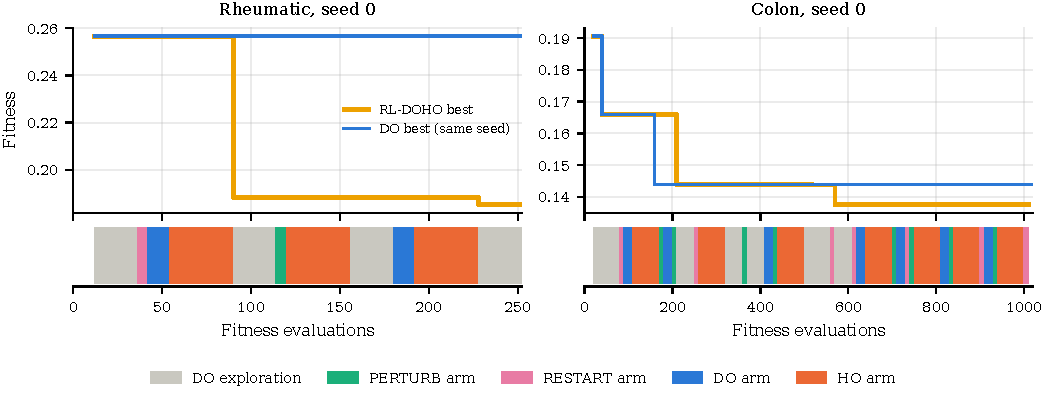
\includegraphics[width=\textwidth]{figs/trace.pdf}
\caption{Best fitness of RL-DOHO and DO for seed 0 on the rheumatic data and on Colon, against evaluations used, with RL-DOHO's action at each step (bottom). On the rheumatic data DO never improves on its initial best with this seed.}
\label{fig:trace}
\end{figure*}

The extension runs show the same picture. The Q-learning controller made 10, 35 and 33 decisions per run on the clinical, gene and tabular data and spread them over all four arms (averaged over runs: DO 33--35\%, PERTURB 27--33\%, RESTART 16--20\%, HO 17--19\%).

\subsection{The intervention layer on GA and HO (H6)}\label{sec:addon}
Table~\ref{tab:addon} and Fig.~\ref{fig:addonk}(a) compare the GA and HO with and without the intervention layer.
\begin{itemize}
\item \textbf{HO+SI against HO:} lower fitness in 71 runs and higher in 29 (Holm $p<0.001$). The gain came mostly from the tabular data (40 against 8), with a weaker trend on gene data (30 against 16, $p=0.054$) and none on the clinical data (1 against 5). HO+SI had the lower mean fitness on 8 of the 11 datasets, by up to 16\% (Colon, Glioma, Dermatology).
\item \textbf{GA+SI against the GA:} no difference (45 against 49), on every data type.
\item \textbf{Test accuracy} did not change in either case (HO+SI 39 against 35, GA+SI 34 against 32).
\item \textbf{Against RL-DOHO}, HO+SI was ahead in 61 runs and behind in 47 ($p=0.21$), and GA+SI was ahead in 85 and behind in 25 ($p<0.001$).
\end{itemize}
HO+SI stalled less often than GA+SI and made fewer decisions (4, 12 and 13 per run on the clinical, gene and tabular data, against 15, 47 and 48). Of the fitness reduction achieved during HO+SI's interventions, 69\% came from PERTURB, 27\% from the HO arm and 4\% from RESTART. For GA+SI the GA arm produced 57\% and PERTURB 42\%.

\begin{table*}[t]
\centering
\caption{The intervention layer on the GA and HO. Top: mean fitness per data type and mean number of selected features over all 110 runs. Bottom: W/T/L for the first-named method on fitness per data type and over all runs, with sign-test $p$ (Holm-corrected over the two H6 comparisons in the first two rows), and on test accuracy.}
\label{tab:addon}
\footnotesize
\setlength{\tabcolsep}{4pt}
\begin{tabular}{@{}lcccc@{}}
\toprule
Method & Clinical & Gene expression & Medical tabular & Features (all) \\
\midrule
RL-DOHO & 0.1832 & 0.0786 & 0.1494 & 78.7 \\
GA & 0.1821 & 0.0616 & 0.1309 & 62.4 \\
GA+SI & 0.1822 & 0.0627 & 0.1321 & 57.9 \\
HO & 0.1838 & 0.0816 & 0.1534 & 52.7 \\
HO+SI & 0.1839 & 0.0738 & 0.1427 & 54.1 \\
\bottomrule
\end{tabular}

\vspace{2mm}
\begin{tabular}{@{}lccccccc@{}}
\toprule
& \multicolumn{5}{c}{Fitness} & \multicolumn{2}{c}{Test accuracy} \\
\cmidrule(lr){2-6}\cmidrule(l){7-8}
Comparison & Clinical (10) & Gene (50) & Tabular (50) & All (110) & $p$ & All (110) & $p$ \\
\midrule
GA+SI vs.\ GA & 2/5/3 & 25/0/25 & 18/11/21 & 45/16/49 & 0.757 & 34/44/32 & 0.902 \\
HO+SI vs.\ HO & 1/4/5 & 30/4/16 & 40/2/8 & 71/10/29 & \textbf{$<$0.001} & 39/36/35 & 0.728 \\
\midrule
RL-DOHO vs.\ GA+SI & 2/0/8 & 16/0/34 & 7/0/43 & 25/0/85 & \textbf{$<$0.001} & 42/13/55 & 0.223 \\
RL-DOHO vs.\ HO+SI & 6/1/3 & 22/1/27 & 19/0/31 & 47/2/61 & 0.211 & 51/10/49 & 0.920 \\
\bottomrule
\end{tabular}
\end{table*}

\begin{figure*}[t]
\centering
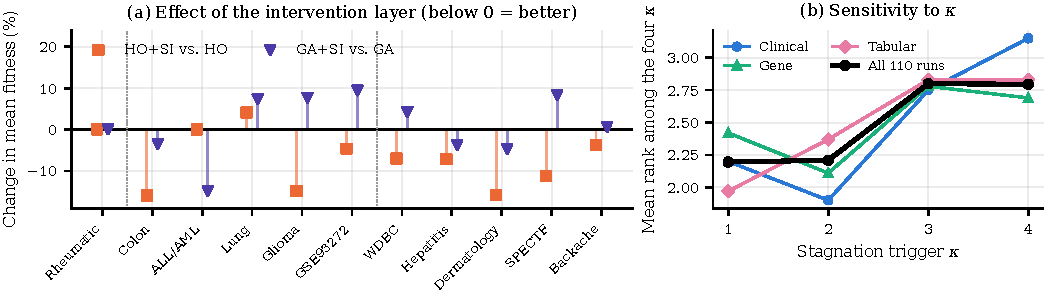
\includegraphics[width=\textwidth]{figs/addon_kappa.pdf}
\caption{(a) Change in mean fitness when the intervention layer is added to HO and to the GA, per dataset (negative is better); dotted lines separate the clinical, gene-expression and tabular datasets. (b) Mean per-run rank of RL-DOHO's fitness among the four values of the stagnation trigger $\kappa$, by data type and over all 110 runs.}
\label{fig:addonk}
\end{figure*}

\subsection{Sensitivity to the stagnation trigger (H7)}\label{sec:kappa}
Table~\ref{tab:kappa} and Fig.~\ref{fig:addonk}(b) vary $\kappa$, the number of stalled iterations before an intervention.
\begin{itemize}
\item The Friedman test over $\kappa\in\{1,2,3,4\}$ is significant ($\chi^2=23.84$, $p<0.001$), so H7 is rejected.
\item $\kappa=1$ and the default $\kappa=2$ were level (mean ranks 2.20 and 2.21; 54 against 50 runs). Waiting longer was worse: $\kappa=3$ lost to $\kappa=2$ in 71 runs and won in 38 ($p=0.002$), and $\kappa=4$ lost in 70 and won in 35 ($p<0.001$).
\item By mean rank, $\kappa=3$ and $\kappa=4$ were worse than $\kappa=2$ on every data type, although the per-type Friedman tests were significant only on gene ($p=0.040$) and tabular data ($p=0.001$). On the tabular data $\kappa=1$ was also better than $\kappa=2$ (31 against 17 runs, $p=0.059$; mean fitness 0.1422 against 0.1494).
\item Test accuracy did not differ between any value of $\kappa$ and the default.
\end{itemize}
The default was fixed before these runs, so the sweep confirms it rather than tuning it.

\begin{table}[t]
\centering
\caption{Sensitivity to the stagnation trigger $\kappa$: mean fitness per data type, mean per-run rank among the four values over 110 runs (Friedman $p<0.001$), and W/T/L against the default $\kappa=2$ with sign-test $p$.}
\label{tab:kappa}
\footnotesize
\setlength{\tabcolsep}{2.6pt}
\begin{tabular}{@{}lcccccc@{}}
\toprule
& \multicolumn{3}{c}{Mean fitness} & & \multicolumn{2}{c}{vs.\ $\kappa=2$} \\
\cmidrule(lr){2-4}\cmidrule(l){6-7}
$\kappa$ & Clinical & Gene & Tabular & Rank & W/T/L & $p$ \\
\midrule
$\kappa=1$ & 0.1836 & 0.0793 & 0.1422 & \textbf{2.20} & 54/6/50 & 0.769 \\
$\kappa=2$ (default) & 0.1832 & 0.0786 & 0.1494 & 2.21 & -- & -- \\
$\kappa=3$ & 0.1855 & 0.0910 & 0.1490 & 2.80 & 38/1/71 & \textbf{0.002} \\
$\kappa=4$ & 0.1857 & 0.0882 & 0.1525 & 2.80 & 35/5/70 & \textbf{$<$0.001} \\
\bottomrule
\end{tabular}
\end{table}

\subsection{Repeated clinical splits (H8)}\label{sec:splits}
Table~\ref{tab:splits} repeats the clinical comparison on two further train/test splits.
\begin{itemize}
\item \textbf{RL-DOHO did about as well on split 1 as on the original split, and worse on split 2.} Its average per-run fitness rank among the 13 methods was 5.2 on the original split, 5.3 on split 1 and 9.2 on split 2. On split 2 the best subset found by any run (fitness 0.1785) was found easily: HO and LASSO reached it in all five runs, HO+SI in four and the GA in three, and RL-DOHO in none.
\item \textbf{H8:} over the 15 paired runs, RL-DOHO's fitness differed significantly only from DO (15 against 0) and the full feature set (14 against 1). The GA was ahead in 12 runs and behind in 3 (unadjusted $p=0.035$, Holm $p=0.35$); all other comparisons were closer.
\item \textbf{Test accuracy} differed significantly only from DO. Apart from DO and BGWO, the methods' mean test accuracy lay within 0.4 percentage points of each other on each new split, and RL-DOHO's per-run test-accuracy rank was 5.67, fourth of 13.
\item \textbf{Within the DO--HO family}, HO had the better average rank on these splits (1.53 against 2.03 for RL-DOHO).
\end{itemize}

\begin{table*}[t]
\centering
\caption{Repeated clinical splits: mean fitness and test accuracy (\%) over seeds 0--4 on the original split and two new splits, mean per-run rank over the 15 runs (1 = best of 13), and W/T/L of RL-DOHO against each method on fitness. Best value per column in bold.}
\label{tab:splits}
\footnotesize
\setlength{\tabcolsep}{4pt}
\begin{tabular}{@{}lccccccccc@{}}
\toprule
& \multicolumn{3}{c}{Fitness} & \multicolumn{3}{c}{Test accuracy} & \multicolumn{2}{c}{Rank} & \\
\cmidrule(lr){2-4}\cmidrule(lr){5-7}\cmidrule(lr){8-9}
Method & Original & Split 1 & Split 2 & Original & Split 1 & Split 2 & Fitness & Test acc. & W/T/L \\
\midrule
\textbf{RL-DOHO} & 0.1837 & 0.1852 & 0.1820 & 84.50 & \textbf{84.68} & 83.08 & 6.57 & 5.67 & -- \\
DO & 0.2368 & 0.2303 & 0.2325 & 79.12 & 79.37 & 78.15 & 12.93 & 12.93 & 15/0/0 \\
HO & 0.1843 & 0.1851 & \textbf{0.1785} & 84.32 & 84.63 & 82.97 & 4.50 & 7.50 & 5/1/9 \\
DOHO & 0.1856 & 0.1865 & 0.1804 & 84.46 & 84.64 & 83.04 & 8.27 & 6.73 & 8/2/5 \\
\midrule
GA & \textbf{0.1821} & \textbf{0.1849} & 0.1794 & 84.41 & 84.68 & 83.12 & \textbf{3.80} & 5.20 & 3/0/12 \\
BPSO & 0.1831 & 0.1854 & 0.1794 & 84.60 & 84.51 & 83.01 & 5.27 & 7.13 & 5/2/8 \\
BGWO & 0.1905 & 0.1937 & 0.1836 & 83.65 & 83.30 & 83.11 & 9.37 & 7.70 & 11/0/4 \\
\midrule
GA+SI & 0.1821 & 0.1852 & 0.1793 & 84.57 & 84.54 & \textbf{83.28} & 4.40 & 5.53 & 3/2/10 \\
HO+SI & 0.1836 & 0.1856 & 0.1786 & 84.39 & 84.60 & 83.06 & 4.80 & 7.30 & 5/2/8 \\
\midrule
LASSO & 0.1868 & 0.1858 & \textbf{0.1785} & 84.92 & 84.57 & 82.97 & 6.67 & 5.87 & 8/0/7 \\
mRMR & 0.1849 & 0.1850 & 0.1799 & 84.49 & 84.65 & 82.92 & 6.20 & 6.67 & 4/4/7 \\
ReliefF & 0.1854 & 0.1855 & 0.1790 & \textbf{84.97} & 84.64 & 83.14 & 6.73 & \textbf{3.80} & 9/0/6 \\
All features & 0.1884 & 0.1873 & 0.1854 & 83.97 & 84.38 & 83.08 & 11.50 & 8.97 & 14/0/1 \\
\bottomrule
\end{tabular}
\end{table*}

\subsection{Cost}
Every method received the same budget of fitness evaluations, but the budget counts repeated subsets too, and repeated subsets are served from the cache. A run's real cost is therefore driven by the number of distinct subsets it evaluates (Table~\ref{tab:cost}).
\begin{itemize}
\item On the new clinical splits, RL-DOHO evaluated 83 distinct subsets per run, against 131 for HO, 132 for the GA and 245 for binary PSO. At about 3.6~s per new subset on the free Colab runtime we used, that is roughly 5, 8, 8 and 15 minutes per run from an empty cache.
\item On the tabular data the pattern was the same (381 against 596, 633 and 1,018 subsets).
\item Fewer distinct subsets also means less exploration. DO evaluated the fewest and was the weakest method, and binary GWO, which also evaluated few, ranked well on the tabular data but poorly on the clinical splits. The count is therefore a cost advantage, not a quality signal.
\item The algorithms' own overhead was below 1.5~ms per evaluation for every method, even at $D=7{,}129$, which is negligible next to a fitness evaluation (about 20~ms for the tabular KNN and 3.6~s for the clinical models).
\end{itemize}

\begin{table}[t]
\centering
\caption{Cost: mean number of distinct subsets evaluated per run on the two new clinical splits (budget 252) and the tabular datasets (budget 1,020), and algorithm overhead in milliseconds per fitness evaluation on a near-free fitness function, by number of features $D$.}
\label{tab:cost}
\footnotesize
\setlength{\tabcolsep}{3pt}
\begin{tabular}{@{}lcccccc@{}}
\toprule
& \multicolumn{2}{c}{Distinct subsets} & \multicolumn{4}{c}{Overhead (ms/evaluation)} \\
\cmidrule(lr){2-3}\cmidrule(l){4-7}
Method & Clinical & Tabular & $D=14$ & 44 & 2,000 & 7,129 \\
\midrule
RL-DOHO & 83 & 381 & 0.08 & 0.06 & 0.26 & 0.77 \\
DO & 13 & 24 & 0.03 & 0.03 & 0.31 & 1.41 \\
HO & 131 & 596 & 0.06 & 0.06 & 0.12 & 0.26 \\
DOHO & 77 & 290 & 0.05 & 0.04 & 0.21 & 0.62 \\
\midrule
GA & 132 & 633 & 0.05 & 0.04 & 0.09 & 0.19 \\
BPSO & 245 & 1018 & 0.02 & 0.02 & 0.09 & 0.27 \\
BGWO & 54 & 237 & 0.08 & 0.08 & 0.20 & 0.48 \\
GA+SI & 171 & 771 & 0.08 & 0.07 & 0.12 & 0.24 \\
HO+SI & 140 & 656 & 0.07 & 0.07 & 0.14 & 0.27 \\
\bottomrule
\end{tabular}
\end{table}


\subsection{A second classifier (H9)}\label{sec:svm}
Table~\ref{tab:svm} repeats the tabular benchmark with an SVM in place of 5-NN.
\begin{itemize}
\item \textbf{The ranking of the methods barely changed.} The mean per-run fitness ranks of the 11 methods under the two classifiers had a Spearman correlation of 0.99; only mRMR and ReliefF swapped places. The GA ranked first (1.58), followed by binary PSO (3.19), binary GWO (3.53), RL-DOHO (3.81) and HO (4.40).
\item \textbf{H9a--H9d replicated.} RL-DOHO beat DO in all 50 runs, was ahead of HO in 32 and behind in 18 ($p=0.065$), and trailed the GA (5 against 43). The intervention layer again improved HO (37 against 8, $p<0.001$) and left the GA unchanged (16 against 17, with 17 ties).
\item \textbf{H9e:} PERTURB alone again reached lower fitness than the full arm set, in 41 runs against 8 ($p<0.001$), on four of the five datasets by at least 8 runs to 2. It did so on WDBC, Dermatology and SPECTF too, so the advantage does not depend on the two weakest datasets.
\item \textbf{Within the DO--HO family}, RL-DOHO had the best average rank (1.54, against 1.79 for HO).
\item \textbf{Test scores:} the SVM's mean test balanced accuracy was similar to 5-NN's (51.8--96.3\% against 53.6--95.5\% across the datasets), and no pooled test-accuracy comparison with RL-DOHO was significant after correction.
\end{itemize}

\begin{table}[t]
\centering
\caption{Medical tabular datasets with an SVM and with 5-NN as the classifier (50 paired runs each, same splits and seeds): W/T/L for the first-named method on fitness and unadjusted two-sided sign-test $p$. Bold: $p<0.05$.}
\label{tab:svm}
\footnotesize
\setlength{\tabcolsep}{2.6pt}
\begin{tabular}{@{}lcccc@{}}
\toprule
& \multicolumn{2}{c}{SVM} & \multicolumn{2}{c}{5-NN} \\
\cmidrule(lr){2-3}\cmidrule(l){4-5}
Comparison & W/T/L & $p$ & W/T/L & $p$ \\
\midrule
RL-DOHO vs.\ DO & 50/0/0 & \textbf{$<$0.001} & 49/0/1 & \textbf{$<$0.001} \\
RL-DOHO vs.\ HO & 32/0/18 & 0.065 & 30/0/20 & 0.203 \\
RL-DOHO vs.\ DOHO & 40/2/8 & \textbf{$<$0.001} & 35/0/15 & \textbf{0.007} \\
GA vs.\ RL-DOHO & 43/2/5 & \textbf{$<$0.001} & 45/1/4 & \textbf{$<$0.001} \\
RL-DOHO vs.\ BPSO & 20/3/27 & 0.382 & 20/0/30 & 0.203 \\
RL-DOHO vs.\ BGWO & 21/2/27 & 0.471 & 20/0/30 & 0.203 \\
RL-DOHO vs.\ LASSO & 41/0/9 & \textbf{$<$0.001} & 38/0/12 & \textbf{$<$0.001} \\
\midrule
HO+SI vs.\ HO & 37/5/8 & \textbf{$<$0.001} & 40/2/8 & \textbf{$<$0.001} \\
GA+SI vs.\ GA & 16/17/17 & 1.000 & 18/11/21 & 0.749 \\
PERTURB only vs.\ RL-DOHO & 41/1/8 & \textbf{$<$0.001} & 39/3/8 & \textbf{$<$0.001} \\
\bottomrule
\end{tabular}
\end{table}

\subsection{Sensitivity to the operator implementation}
An earlier version of this study used simplified three-phase versions of the DO and HO update rules, a dense start on all datasets, the old reward and a budget defined in iterations. Table~\ref{tab:sens} compares the two versions on the six datasets of the main study, with the same splits and seeds.
\begin{itemize}
\item \textbf{Simplified rules:} RL-DOHO was ahead of DO in 41 of the 60 runs and behind in 13. It was level with HO (30 against 29) and behind the GA (20 against 39).
\item \textbf{Published rules:} the corresponding figures are 54 against 3, 28 against 29 and 18 against 40.
\item \textbf{The conclusions about the DO--HO family and the GA are unchanged:} clearly better than DO, level with HO, behind the GA. With the published rules the gap to DO widens, partly because the published DO stalls on the clinical problem.
\item \textbf{The comparison with binary PSO and GWO reversed.} Under v1, RL-DOHO was behind both (25 against 34 and 22 against 38 runs); under v2 it was ahead (50 against 8 and 47 against 13). This change most likely comes from the sparse start, which RL-DOHO keeps and the two baselines drift away from.
\item \textbf{Gene data:} the new configuration reduced the subsets of the DO--HO family from about 2,100 genes to 99--157 and lowered their fitness substantially. Their mean test accuracy fell by 1.2--3.2 points, while that of the GA, BPSO and BGWO changed by about 0.2 points or less.
\item \textbf{GA, BPSO and BGWO} also improved in fitness under the sparse start.
\end{itemize}

\begin{table*}[t]
\centering
\caption{Sensitivity analysis: mean fitness and test accuracy (\%) of the wrapper methods under the earlier configuration (v1: simplified DO/HO rules, dense start, old reward) and the final one (v2), and mean number of selected genes on gene data. On the clinical data the GA, BPSO and BGWO runs are shared by both versions.}
\label{tab:sens}
\footnotesize
\setlength{\tabcolsep}{4pt}
\begin{tabular}{@{}lcccccccccc@{}}
\toprule
& \multicolumn{4}{c}{Rheumatic} & \multicolumn{4}{c}{Gene expression (5 datasets)} & \multicolumn{2}{c}{Genes selected} \\
\cmidrule(lr){2-5}\cmidrule(lr){6-9}\cmidrule(l){10-11}
Method & Fit.\ v1 & Fit.\ v2 & Acc.\ v1 & Acc.\ v2 & Fit.\ v1 & Fit.\ v2 & Acc.\ v1 & Acc.\ v2 & v1 & v2 \\
\midrule
RL-DOHO & 0.1845 & 0.1832 & 84.3 & 84.3 & 0.1396 & 0.0786 & 84.4 & 83.2 & 2098 & 157 \\
DO & 0.1871 & 0.2280 & 84.1 & 80.0 & 0.1443 & 0.1113 & 83.8 & 81.2 & 2114 & 124 \\
HO & 0.1880 & 0.1838 & 83.8 & 84.3 & 0.1382 & 0.0816 & 85.0 & 81.8 & 2110 & 99 \\
DOHO & 0.1882 & 0.1857 & 84.0 & 84.5 & 0.1403 & 0.0966 & 84.7 & 82.0 & 2114 & 115 \\
\midrule
GA & 0.1821 & (same) & 84.4 & (same) & 0.1432 & 0.0616 & 83.5 & 83.5 & 2006 & 121 \\
BPSO & 0.1828 & (same) & 84.5 & (same) & 0.1344 & 0.1192 & 83.8 & 83.6 & 2122 & 670 \\
BGWO & 0.1894 & (same) & 83.8 & (same) & 0.1362 & 0.1014 & 83.8 & 83.9 & 2031 & 772 \\
\bottomrule
\end{tabular}
\end{table*}



%% ======================================================================
\section{Discussion}\label{sec:discussion}

\subsection{Why RL-DOHO improves on DO}
With the binary encoding used here, a feature changes only when its coordinate crosses zero. The published DO's landing stage pulls the whole population to within small Lévy steps of the elite in every iteration. On a 14-feature problem this almost always reproduces the elite's subset, which is why DO improved on its initial best in only one clinical run. On gene data, with thousands of coordinates, the heavy tails of the Lévy steps do flip some features, and DO improved in 48 of 50 runs, but slowly. RL-DOHO's interventions supply exactly what DO lacks under this encoding: new subsets near the best one (PERTURB), new subsets elsewhere (RESTART), and HO's greedy, randomized moves. The ablation supports this reading: removing the interventions made results worse in 103 of 110 runs. This result depends on the encoding and on the Lévy scale of the original paper (0.01); a transfer function with more spread, or larger steps, might let DO move more freely.

\subsection{What the interventions contribute}
The add-on experiment separates the interventions from DO. Attached to HO, they improved fitness in 71 of 100 decided runs; attached to the GA, they changed nothing. The difference is not that the GA never stalls: GA+SI made 47--48 intervention decisions per gene or tabular run, against 12--13 for HO+SI. It lies in what the base optimizer does after a stall. A GA generation recombines and mutates good subsets directly in the binary space, and within GA+SI's interventions the GA arm itself produced 57\% of the fitness reduction, so the extra moves largely duplicated what the GA already does. An HO iteration costs about $3N$ evaluations and moves continuous positions relative to a dominant agent; it does not search next to the best subset, which is what PERTURB adds at a cost of $N/2$. The interventions therefore help when they supply a kind of move the base optimizer lacks, rather than wrapper search in general.

Among the interventions, PERTURB, a bit-flip local search around the best subset, is the most useful on low-dimensional data. It produced 69\% of the fitness reduction during HO+SI's interventions (42\% in GA+SI), and PERTURB alone beat the full arm set on the tabular data with both classifiers (39 against 8 runs with 5-NN, 41 against 8 with an SVM) and was ahead on the clinical data too, although not significantly (6 against 2). On gene data, where a few bit flips change little among thousands of features, the full arm set was ahead (30 against 19, not significant), and in RL-DOHO's main gene runs DO exploration steps produced more of the improvement than PERTURB. The $\kappa$ sweep points the same way: intervening after one or two stalled iterations was better than waiting three or four. A practical reading is that a stalled population-based search should be followed quickly by a short local search around its best subset; on our tabular datasets (19--44 features) that local search alone was the better choice overall, although not on every dataset (for example Hepatitis with the SVM, 5 against 4), and on gene data it was not. The fitness advantage of PERTURB alone did not show up in test accuracy (19 against 26 runs with 5-NN, 21 against 22 with an SVM), in line with the other comparisons.

\subsection{Why the controller did not help}
The controller result now holds for three controllers (UCB1, a stateful Q-learner and random selection), two reward designs, three data types and two budgets, so it is unlikely to be an artefact of a single setting. Two factors explain it. First, the arms are complementary rather than ranked. In any given stall several arms are reasonable choices, so a random choice loses little. Second, the decisions are few. At the standard budget the bandit made 9 decisions per clinical run, four of them initial pulls, and about 30 per gene or tabular run; the Q-learner, which has six states to fill, had 10 to 35. That leaves little room for a learned preference to pay off within a run. The Q-learner was, if anything, slightly worse than the bandit, which is consistent with it spending about one in six of its few decisions on random exploration. We therefore describe RL-DOHO's controller as an adaptive selector that costs nothing and removes the need to fix the arm in advance. On our data it delivered no gain over random selection, and the method's benefits should be attributed to the interventions and the initialization. Carrying the controller's learning across runs or datasets, rather than starting each run from zero, is the obvious way to give it more decisions.

\subsection{RL-DOHO, HO and the GA}
RL-DOHO and HO reached statistically indistinguishable fitness (58 against 49 over 110 runs), although RL-DOHO had the better family rank and was rarely the worst of the four. On the repeated clinical splits HO had the better family rank. The GA reached lower fitness than RL-DOHO more often on every data type (85 against 22 overall). Its uniform crossover recombines good subsets directly in the binary space, and with a mutation rate of $1/D$ it stays close to sparse subsets once it starts there; neither property depends on a continuous-to-binary mapping. On test accuracy the GA and RL-DOHO did not differ (48 against 48).

\subsection{Filters, wrappers and optimistic fitness}
The filters' standing depended on the data type. On gene data LASSO reached lower fitness than every wrapper on every dataset, and mRMR did so on ALL/AML and Lung. On the tabular and clinical data, with 14--44 features, the wrappers led and LASSO, mRMR and ReliefF trailed RL-DOHO. Part of the filters' fitness advantage on gene data is optimistic, however. Their subset size was chosen by minimizing the same cross-validated score that is reported as fitness, the selection bias described by Ambroise and McLachlan~\cite{ambroise2002}. Glioma shows the effect most clearly: LASSO had the best fitness and the worst test accuracy. On held-out data the differences shrink: in the pooled tests over all 110 runs no test-accuracy difference survived correction, and LASSO's lead over RL-DOHO on macro-F1 was the only test-score difference that did.

\subsection{Clinical data}
On the rheumatic data all methods except the published DO reached test accuracy within about 1.1 points of each other on the original split and, apart from BGWO, within 0.4 points on each new split, and the best subsets were found by many methods. The dataset is too easy to separate the better search methods, which is also why the intervention layer made no difference to HO or the GA there. The two variables that RL-DOHO, the GA, BPSO and BGWO mostly dropped, anti-dsDNA and anti-Sm, are the two with the most missing values (39\% and 43\%). Their low value in this dataset may therefore reflect missingness and mode imputation rather than clinical irrelevance. Where fitness evaluations are expensive, as with the boosted models used here, RL-DOHO's smaller number of distinct subsets is a practical advantage at equal test accuracy.

\subsection{Limitations}
Several limitations qualify these results. The clinical findings come from a single cohort, now evaluated on three train/test splits with five seeds each, so they describe this cohort rather than rheumatic diagnosis in general, and validation on an external cohort is still needed. The tabular datasets, the add-on experiment, the Q-learning controller, the $\kappa$ sweep and the SVM runs were designed after the main results were known; their hypotheses were fixed before they were run, but the choice of what to test was informed by the earlier findings. The evaluation budgets (252 and 1,020 fitness evaluations) are modest, and only the controllers were examined at a larger budget. Test sets of 15--171 samples on the gene and tabular data make test scores coarse, which is why we give more weight to fitness and to the pooled tests. The tabular benchmark was repeated with an SVM, but the gene-expression and clinical data were each evaluated with a single classifier configuration (5-NN, and XGBoost with gradient boosting on a 4,000-patient subsample), and no classifier was tuned. RL-DOHO's settings other than $\kappa$, including $\varepsilon$ and the UCB constant, and the Q-learning settings were fixed rather than tuned, which keeps the comparison even but leaves their sensitivity open. Our DO and HO follow the published equations, although the original papers leave some details open (such as the random-group size in HO), so other implementations may behave differently. The cost figures come from one shared cloud runtime, and the per-evaluation cost on the clinical data was recorded on one split only. We did not compare against recent binary HO variants such as Q2HO-MFTV~\cite{hashjin2025q2ho}, which we did not reimplement. Two of the tabular datasets (Backache and Hepatitis) are close to chance for 5-NN; Table~\ref{tab:weak} shows which conclusions depend on them. Finally, the filter methods chose their subset size on the same cross-validated score that is reported as fitness, which favours them on that measure, and the pooled sign tests treat runs on the same dataset as independent and combine datasets of different size and difficulty. They are best read together with the per-dataset results and the dataset-level ranks, on which RL-DOHO is separated only from DO and the full feature set.

%% ======================================================================
\section{Conclusion}
We presented RL-DOHO, a DO--HO hybrid. It runs the published DO while the search improves and, after two stagnant iterations, applies one of four interventions chosen by a UCB1 bandit, with tabu memory, a gain-based reward and a sparse start for high-dimensional data. Across eleven datasets and ten seeds, with equal evaluation budgets and hypotheses fixed in advance:
\begin{itemize}
\item RL-DOHO reached lower fitness than the published DO, a fixed DO-then-HO hybrid and binary PSO significantly more often than not.
\item It was level with the published HO, had a slightly better average rank in the DO--HO family and was its worst member in 2 of 110 runs, although HO ranked better on the repeated clinical splits.
\item A GA reached lower fitness more often, and no test-accuracy difference was significant after correction.
\item The same intervention layer improved HO but not the GA, whose own generations already supply the local moves the layer adds.
\item How the intervention was chosen did not matter: UCB1, Q-learning and random selection were level, and intervening early ($\kappa\le2$) was better than waiting. On the tabular datasets (19--44 features), a bit-flip search around the best subset alone beat the full set of interventions; on gene data, with thousands of features, it did not (the full set was ahead, not significantly).
\item An SVM in place of 5-NN barely changed the ranking of the methods on the tabular data and reproduced the main comparisons there.
\item Over three clinical train/test splits, RL-DOHO differed significantly only from DO and the full feature set. On the clinical and tabular data it needed 35--40\% fewer distinct fitness evaluations than HO or the GA.
\end{itemize}
Future work should test the method on more clinical cohorts with external validation, let the controller learn across runs rather than within one, and examine binary encodings under which the published DO can move more freely.

\section*{Data and Code Availability}
The rheumatic dataset is openly available (CC BY 4.0) from the source cited in~\cite{mahdi2025data}. The microarray datasets are from the scikit-feature repository~\cite{li2017fs}, GSE93272 is available from the NCBI Gene Expression Omnibus, and the five tabular datasets are from PMLB~\cite{olson2017pmlb}. The notebooks, per-run results, figures and analysis scripts used in this study are available at \url{https://github.com/adj-04/rl-doho}.

\begin{thebibliography}{00}

\bibitem{kohavi1997} R. Kohavi and G. H. John, ``Wrappers for feature subset selection,'' \textit{Artif. Intell.}, vol. 97, no. 1--2, pp. 273--324, 1997, doi: 10.1016/S0004-3702(97)00043-X.

\bibitem{xue2016} B. Xue, M. Zhang, W. N. Browne, and X. Yao, ``A survey on evolutionary computation approaches to feature selection,'' \textit{IEEE Trans. Evol. Comput.}, vol. 20, no. 4, pp. 606--626, 2016, doi: 10.1109/TEVC.2015.2504420.

\bibitem{zhao2022do} S. Zhao, T. Zhang, S. Ma, and M. Chen, ``Dandelion Optimizer: A nature-inspired metaheuristic algorithm for engineering applications,'' \textit{Eng. Appl. Artif. Intell.}, vol. 114, Art. no. 105075, 2022, doi: 10.1016/j.engappai.2022.105075.

\bibitem{amiri2024ho} M. H. Amiri, N. Mehrabi Hashjin, M. Montazeri, S. Mirjalili, and N. Khodadadi, ``Hippopotamus optimization algorithm: a novel nature-inspired optimization algorithm,'' \textit{Sci. Rep.}, vol. 14, Art. no. 5032, 2024, doi: 10.1038/s41598-024-54910-3.

\bibitem{auer2002} P. Auer, N. Cesa-Bianchi, and P. Fischer, ``Finite-time analysis of the multiarmed bandit problem,'' \textit{Mach. Learn.}, vol. 47, no. 2--3, pp. 235--256, 2002, doi: 10.1023/A:1013689704352.

\bibitem{sutton2018} R. S. Sutton and A. G. Barto, \textit{Reinforcement Learning: An Introduction}, 2nd ed. Cambridge, MA, USA: MIT Press, 2018.

\bibitem{mahdi2025data} M. F. Mahdi, A. Jahani, and D. H. Abd, ``Diagnosis of rheumatic and autoimmune diseases dataset,'' \textit{Data Brief}, vol. 60, Art. no. 111623, 2025, doi: 10.1016/j.dib.2025.111623.

\bibitem{kennedy1997} J. Kennedy and R. C. Eberhart, ``A discrete binary version of the particle swarm algorithm,'' in \textit{Proc. IEEE Int. Conf. Syst., Man, Cybern.}, vol. 5, 1997, pp. 4104--4108, doi: 10.1109/ICSMC.1997.637339.

\bibitem{mirjalili2014gwo} S. Mirjalili, S. M. Mirjalili, and A. Lewis, ``Grey wolf optimizer,'' \textit{Adv. Eng. Softw.}, vol. 69, pp. 46--61, 2014, doi: 10.1016/j.advengsoft.2013.12.007.

\bibitem{emary2016bgwo} E. Emary, H. M. Zawbaa, and A. E. Hassanien, ``Binary grey wolf optimization approaches for feature selection,'' \textit{Neurocomputing}, vol. 172, pp. 371--381, 2016, doi: 10.1016/j.neucom.2015.06.083.

\bibitem{mafarja2017} M. M. Mafarja and S. Mirjalili, ``Hybrid whale optimization algorithm with simulated annealing for feature selection,'' \textit{Neurocomputing}, vol. 260, pp. 302--312, 2017, doi: 10.1016/j.neucom.2017.04.053.

\bibitem{wolpert1997} D. H. Wolpert and W. G. Macready, ``No free lunch theorems for optimization,'' \textit{IEEE Trans. Evol. Comput.}, vol. 1, no. 1, pp. 67--82, 1997, doi: 10.1109/4235.585893.

\bibitem{ramadhani2025} S. Ramadhani, L. Handayani, T. F. Ng, S. Dzulkifly, R. Ariffin, H. Budiman, and S. L. Wang, ``Feature selection optimisation for cancer classification based on evolutionary algorithms: An extensive review,'' \textit{Comput. Model. Eng. Sci.}, vol. 143, no. 3, pp. 2711--2765, 2025, doi: 10.32604/cmes.2025.062709.

\bibitem{zhao2026review} S. Zhao, J. Song, T. Zhang, and J. He, ``Dandelion Optimizer (DO): A review, theory, variants, and applications,'' \textit{Arch. Comput. Methods Eng.}, vol. 33, no. 2, pp. 2553--2577, 2026, doi: 10.1007/s11831-025-10385-7.

\bibitem{tang2024psodo} W. Tang, L. Cao, Y. Chen, B. Chen, and Y. Yue, ``Solving engineering optimization problems based on multi-strategy particle swarm optimization hybrid dandelion optimization algorithm,'' \textit{Biomimetics}, vol. 9, no. 5, Art. no. 298, 2024, doi: 10.3390/biomimetics9050298.

\bibitem{kiziloluk2024} S. Kiziloluk, M. Yildirim, H. Bingol, and B. Alatas, ``Multi-feature fusion and dandelion optimizer based model for automatically diagnosing the gastrointestinal diseases,'' \textit{PeerJ Comput. Sci.}, vol. 10, Art. no. e1919, 2024, doi: 10.7717/peerj-cs.1919.

\bibitem{alzakari2024} S. A. Alzakari, M. Maashi, S. Alahmari, M. A. Arasi, A. A. K. Alharbi, and A. Sayed, ``Towards laryngeal cancer diagnosis using Dandelion Optimizer Algorithm with ensemble learning on biomedical throat region images,'' \textit{Sci. Rep.}, vol. 14, Art. no. 19713, 2024, doi: 10.1038/s41598-024-70525-0.

\bibitem{pei2025} S. Pei, G. Sun, and L. Tong, ``An improved hippopotamus optimization algorithm based on adaptive development and solution diversity enhancement,'' \textit{PeerJ Comput. Sci.}, vol. 11, Art. no. e2901, 2025, doi: 10.7717/peerj-cs.2901.

\bibitem{ardiyansa2025} S. A. Ardiyansa, M. Muslikh, and A. R. Alghofari, ``Binary hippopotamus algorithm with random forest for optimizing feature selection problem,'' \textit{Numer. Algebra Control Optim.}, vol. 15, no. 4, pp. 1176--1191, 2025, doi: 10.3934/naco.2025009.

\bibitem{yuan2025msho} X. Yuan, L. Yao, T. Zhang, Q. Chen, and G. Li, ``An effective method for solving feature selection problems based on multi-strategy Hippo optimization algorithm,'' \textit{J. Comput. Des. Eng.}, vol. 12, no. 8, pp. 193--251, 2025, doi: 10.1093/jcde/qwaf073.

\bibitem{hashjin2025q2ho} N. Mehrabi Hashjin, M. H. Amiri, A. Beheshti, and M. Khanian Najafabadi, ``Q2HO-MFTV: A binary hippopotamus optimization algorithm for feature selection with a brief review of binary optimization,'' \textit{Knowl.-Based Syst.}, vol. 327, Art. no. 114119, 2025, doi: 10.1016/j.knosys.2025.114119.

\bibitem{karafotias2015} G. Karafotias, M. Hoogendoorn, and A. E. Eiben, ``Parameter control in evolutionary algorithms: Trends and challenges,'' \textit{IEEE Trans. Evol. Comput.}, vol. 19, no. 2, pp. 167--187, 2015, doi: 10.1109/TEVC.2014.2308294.

\bibitem{fialho2010} \'A. Fialho, L. Da Costa, M. Schoenauer, and M. Sebag, ``Analyzing bandit-based adaptive operator selection mechanisms,'' \textit{Ann. Math. Artif. Intell.}, vol. 60, no. 1--2, pp. 25--64, 2010, doi: 10.1007/s10472-010-9213-y.

\bibitem{hu2023rlgwo} Z. Hu and X. Yu, ``Reinforcement learning-based comprehensive learning grey wolf optimizer for feature selection,'' \textit{Appl. Soft Comput.}, vol. 149, Art. no. 110959, 2023, doi: 10.1016/j.asoc.2023.110959.

\bibitem{karimi2023} M. Karimi-Mamaghan, M. Mohammadi, B. Pasdeloup, and P. Meyer, ``Learning to select operators in meta-heuristics: An integration of Q-learning into the iterated greedy algorithm for the permutation flowshop scheduling problem,'' \textit{Eur. J. Oper. Res.}, vol. 304, no. 3, pp. 1296--1330, 2023, doi: 10.1016/j.ejor.2022.03.054.

\bibitem{mahdi2025fuzzy} M. F. Mahdi, A. Jahani, and D. H. Abd, ``Fuzzy evaluation and explainable machine learning for diagnosis of rheumatic and autoimmune diseases,'' \textit{PeerJ Comput. Sci.}, vol. 11, Art. no. e3096, 2025, doi: 10.7717/peerj-cs.3096.

\bibitem{karadayi2025} P. Karaday{\i} Ata\c{s}, ``A novel clustered-based binary grey wolf optimizer to solve the feature selection problem for uncovering the genetic links between non-Hodgkin lymphomas and rheumatologic diseases,'' \textit{Health Inf. Sci. Syst.}, vol. 13, Art. no. 34, 2025, doi: 10.1007/s13755-025-00350-w.

\bibitem{li2017fs} J. Li, K. Cheng, S. Wang, F. Morstatter, R. P. Trevino, J. Tang, and H. Liu, ``Feature selection: A data perspective,'' \textit{ACM Comput. Surv.}, vol. 50, no. 6, Art. no. 94, 2017, doi: 10.1145/3136625.

\bibitem{alon1999} U. Alon, N. Barkai, D. A. Notterman, K. Gish, S. Ybarra, D. Mack, and A. J. Levine, ``Broad patterns of gene expression revealed by clustering analysis of tumor and normal colon tissues probed by oligonucleotide arrays,'' \textit{Proc. Natl. Acad. Sci. USA}, vol. 96, no. 12, pp. 6745--6750, 1999, doi: 10.1073/pnas.96.12.6745.

\bibitem{golub1999} T. R. Golub \textit{et al.}, ``Molecular classification of cancer: Class discovery and class prediction by gene expression monitoring,'' \textit{Science}, vol. 286, no. 5439, pp. 531--537, 1999, doi: 10.1126/science.286.5439.531.

\bibitem{bhattacharjee2001} A. Bhattacharjee \textit{et al.}, ``Classification of human lung carcinomas by mRNA expression profiling reveals distinct adenocarcinoma subclasses,'' \textit{Proc. Natl. Acad. Sci. USA}, vol. 98, no. 24, pp. 13790--13795, 2001, doi: 10.1073/pnas.191502998.

\bibitem{nutt2003} C. L. Nutt \textit{et al.}, ``Gene expression-based classification of malignant gliomas correlates better with survival than histological classification,'' \textit{Cancer Res.}, vol. 63, no. 7, pp. 1602--1607, 2003.

\bibitem{tasaki2018} S. Tasaki \textit{et al.}, ``Multi-omics monitoring of drug response in rheumatoid arthritis in pursuit of molecular remission,'' \textit{Nat. Commun.}, vol. 9, Art. no. 2755, 2018, doi: 10.1038/s41467-018-05044-4.

\bibitem{chen2016xgb} T. Chen and C. Guestrin, ``XGBoost: A scalable tree boosting system,'' in \textit{Proc. 22nd ACM SIGKDD Int. Conf. Knowl. Discov. Data Min.}, 2016, pp. 785--794, doi: 10.1145/2939672.2939785.

\bibitem{chawla2002} N. V. Chawla, K. W. Bowyer, L. O. Hall, and W. P. Kegelmeyer, ``SMOTE: Synthetic minority over-sampling technique,'' \textit{J. Artif. Intell. Res.}, vol. 16, pp. 321--357, 2002, doi: 10.1613/jair.953.

\bibitem{tibshirani1996} R. Tibshirani, ``Regression shrinkage and selection via the lasso,'' \textit{J. R. Stat. Soc. Ser. B}, vol. 58, no. 1, pp. 267--288, 1996, doi: 10.1111/j.2517-6161.1996.tb02080.x.

\bibitem{peng2005} H. Peng, F. Long, and C. Ding, ``Feature selection based on mutual information: Criteria of max-dependency, max-relevance, and min-redundancy,'' \textit{IEEE Trans. Pattern Anal. Mach. Intell.}, vol. 27, no. 8, pp. 1226--1238, 2005, doi: 10.1109/TPAMI.2005.159.

\bibitem{kononenko1994} I. Kononenko, ``Estimating attributes: Analysis and extensions of RELIEF,'' in \textit{Proc. Eur. Conf. Mach. Learn. (ECML)}, LNCS vol. 784, 1994, pp. 171--182, doi: 10.1007/3-540-57868-4\_57.

\bibitem{demsar2006} J. Dem\v{s}ar, ``Statistical comparisons of classifiers over multiple data sets,'' \textit{J. Mach. Learn. Res.}, vol. 7, pp. 1--30, 2006.

\bibitem{friedman1937} M. Friedman, ``The use of ranks to avoid the assumption of normality implicit in the analysis of variance,'' \textit{J. Amer. Statist. Assoc.}, vol. 32, no. 200, pp. 675--701, 1937, doi: 10.1080/01621459.1937.10503522.

\bibitem{wilcoxon1945} F. Wilcoxon, ``Individual comparisons by ranking methods,'' \textit{Biometrics Bull.}, vol. 1, no. 6, pp. 80--83, 1945, doi: 10.2307/3001968.

\bibitem{holm1979} S. Holm, ``A simple sequentially rejective multiple test procedure,'' \textit{Scand. J. Statist.}, vol. 6, no. 2, pp. 65--70, 1979.

\bibitem{nemenyi1963} P. B. Nemenyi, ``Distribution-free multiple comparisons,'' Ph.D. dissertation, Princeton Univ., Princeton, NJ, USA, 1963.

\bibitem{ambroise2002} C. Ambroise and G. J. McLachlan, ``Selection bias in gene extraction on the basis of microarray gene-expression data,'' \textit{Proc. Natl. Acad. Sci. USA}, vol. 99, no. 10, pp. 6562--6566, 2002, doi: 10.1073/pnas.102102699.


\bibitem{watkins1992} C. J. C. H. Watkins and P. Dayan, ``Q-learning,'' \textit{Mach. Learn.}, vol. 8, no. 3--4, pp. 279--292, 1992, doi: 10.1007/BF00992698.

\bibitem{olson2017pmlb} R. S. Olson, W. La Cava, P. Orzechowski, R. J. Urbanowicz, and J. H. Moore, ``PMLB: a large benchmark suite for machine learning evaluation and comparison,'' \textit{BioData Min.}, vol. 10, Art. no. 36, 2017, doi: 10.1186/s13040-017-0154-4.

\bibitem{street1993} W. N. Street, W. H. Wolberg, and O. L. Mangasarian, ``Nuclear feature extraction for breast tumor diagnosis,'' in \textit{Proc. SPIE}, vol. 1905, 1993, pp. 861--870, doi: 10.1117/12.148698.

\bibitem{guvenir1998} H. A. G\"uvenir, G. Demir\"oz, and N. \.Ilter, ``Learning differential diagnosis of erythemato-squamous diseases using voting feature intervals,'' \textit{Artif. Intell. Med.}, vol. 13, no. 3, pp. 147--165, 1998, doi: 10.1016/S0933-3657(98)00028-1.

\bibitem{kurgan2001} L. A. Kurgan, K. J. Cios, R. Tadeusiewicz, M. Ogiela, and L. S. Goodenday, ``Knowledge discovery approach to automated cardiac SPECT diagnosis,'' \textit{Artif. Intell. Med.}, vol. 23, no. 2, pp. 149--169, 2001, doi: 10.1016/S0933-3657(01)00082-3.

\end{thebibliography}

\end{document}
